% ============================================================
% main.tex —— 大连理工大学本科毕业论文主文件
% 论文题目：基于在线评论的消费者多属性态度预测效度研究
%           ——大语言模型提取方法与评论者经验的调节作用
% 编译命令：
%   xelatex main.tex
%   biber main
%   xelatex main.tex
%   xelatex main.tex
% ============================================================

\documentclass[
  12pt,
  a4paper,
  UTF8,
  zihao = -4,        % 全局默认小四号
  scheme = plain,    % 不自动更改标题格式（由preamble手动设置）
]{ctexart}

% 加载格式设置
% ============================================================
% preamble.tex —— 大连理工大学本科毕业论文 LaTeX 格式设置
% 编译方式：xelatex -> biber -> xelatex -> xelatex
% ============================================================

% ---------- 页面尺寸 ----------
\usepackage{geometry}
\geometry{
  paper     = a4paper,
  top       = 35mm,
  bottom    = 25mm,
  left      = 25mm,
  right     = 25mm,
  headsep   = 10mm,
  footskip  = 20mm,
  headheight= 14pt,
}

% ---------- 中英文字体 ----------
\usepackage{fontspec}
\usepackage{xeCJK}
% 中文字体（Windows系统内置）
\setCJKmainfont{SimSun}[
  BoldFont   = SimHei,
  ItalicFont = KaiTi,
  AutoFakeBold = 2,
]
\setCJKsansfont{SimHei}[AutoFakeBold = 2]
\setCJKmonofont{FangSong}
% 华文细黑（封面题目用，AutoFakeBold模拟加粗）
\newfontfamily\xihei{STXihei}[AutoFakeBold=2]
% 英文字体
\setmainfont{Times New Roman}
\setsansfont{Arial}
\setmonofont{Courier New}

% ---------- 字号别名（方便正文调用）----------
% \zihao{-4} = 小四号 = 12pt（正文默认）
% \zihao{4}  = 四号   = 14pt（节标题）
% \zihao{-3} = 小三号 = 15pt（章标题）

% ---------- 行距 ----------
\usepackage{setspace}
\setstretch{1.25}                     % 多倍行距1.25（模板要求）

% ---------- 首行缩进 ----------
\usepackage{indentfirst}
\setlength{\parindent}{2\ccwd}        % 首行缩进2个中文字符

% ---------- 段间距 ----------
\setlength{\parskip}{0pt}

% ---------- 章节标题格式（ctex宏包已在主文件加载）----------
\ctexset{
  % 一级标题：黑体，小三，居左，段后1行
  section = {
    format      = \zihao{-3}\heiti\raggedright,
    beforeskip  = 0pt,
    afterskip   = 22pt,   % 1行 = 小三(15pt)×1.5倍行距 ≈ 22pt
  },
  % 二级标题：黑体，四号，居左
  subsection = {
    format      = \zihao{4}\heiti\raggedright,
    beforeskip  = 6pt,
    afterskip   = 0pt,
  },
  % 三级标题：黑体，小四，居左
  subsubsection = {
    format      = \zihao{-4}\heiti\raggedright,
    beforeskip  = 6pt,
    afterskip   = 0pt,
  },
}

% ---------- 目录格式 ----------
\usepackage{tocloft}
% 目录标题：黑体，小三，居中
\renewcommand{\contentsname}{目\quad 录}
% 一级目录：黑体，小四
\renewcommand{\cftsecfont}{\heiti\zihao{-4}}
\renewcommand{\cftsecpagefont}{\zihao{-4}}
% 二级及以下目录：宋体，小四
\renewcommand{\cftsubsecfont}{\songti\zihao{-4}}
\renewcommand{\cftsubsecpagefont}{\zihao{-4}}
\renewcommand{\cftsubsubsecfont}{\songti\zihao{-4}}
\renewcommand{\cftsubsubsecpagefont}{\zihao{-4}}
\setlength{\cftbeforesecskip}{6pt}

% ---------- 页眉页脚 ----------
\usepackage{fancyhdr}
\pagestyle{fancy}
\fancyhf{}
\fancyhead[C]{\zihao{5}\songti 基于在线评论的消费者多属性态度预测效度研究}
\fancyfoot[C]{\zihao{-5}\songti \thepage}
\renewcommand{\headrulewidth}{0.4pt}
\renewcommand{\footrulewidth}{0pt}

% 纯页码样式（摘要、目录用）
\fancypagestyle{plain}{
  \fancyhf{}
  \fancyfoot[C]{\zihao{-5}\songti \thepage}
  \renewcommand{\headrulewidth}{0pt}
}

% ---------- 参考文献（GB/T 7714-2015）----------
\usepackage[
  backend  = biber,
  style    = gb7714-2015,
  citestyle = gb7714-2015,
  gbpub    = false,
  doi      = false,
  url      = false,
]{biblatex}
\addbibresource{refs/refs01.bib}   % [1]-[10]  态度理论、评论影响
\addbibresource{refs/refs02.bib}   % [11]-[20] 文本信息量、行为意向
\addbibresource{refs/refs03.bib}   % [21]-[30] CMV/效度、ABSA、LLM
\addbibresource{refs/refs04.bib}   % [31]-[41] 中文NLP、消费者专业性
\addbibresource{refs/refs05.bib}   % [42]+  补充文献条目

% ---------- 表格 ----------
\usepackage{booktabs}     % 三线表：\toprule \midrule \bottomrule
\usepackage{longtable}    % 跨页长表格
\usepackage{array}
\usepackage{multirow}
\usepackage{tabularx}
\usepackage{makecell}
\usepackage{threeparttable}  % tablenotes 表格注脚环境

% 表格字体默认小五号
\let\oldtabular\tabular
\renewcommand{\tabular}{\zihao{5}\oldtabular}

% ---------- 图片 ----------
\usepackage{graphicx}
\usepackage{float}
\graphicspath{{figures/}}

% ---------- 图表标题格式 ----------
\usepackage{caption}
\captionsetup{
  font       = {small},             % 宋体五号
  labelsep   = space,
  skip       = 6pt,
}
% 图标题在图下方，表标题在表上方（通过放置位置控制，无需captionsetup）

% 图/表编号格式：图1-1，表2-3
\renewcommand{\thefigure}{\thesection-\arabic{figure}}
\renewcommand{\thetable}{\thesection-\arabic{table}}

% ---------- 数学公式 ----------
\usepackage{amsmath}
\usepackage{amssymb}
\usepackage{amsthm}

% 公式编号格式：(1-1)
\renewcommand{\theequation}{\thesection-\arabic{equation}}

% ---------- tikz（研究框架图）----------
\usepackage{tikz}
\usetikzlibrary{
  shapes.geometric,
  arrows.meta,
  positioning,
  calc,
  fit,
  backgrounds,
  decorations.pathreplacing,
}

% ---------- 超链接（目录可点击）----------
\usepackage[
  colorlinks = true,
  linkcolor  = black,
  citecolor  = black,
  urlcolor   = blue,
  hidelinks,
]{hyperref}

% ---------- 其他常用宏包 ----------
\usepackage{xcolor}
\usepackage{listings}       % 代码块（附录用）
\usepackage{enumitem}       % 列表格式控制
\usepackage{footnotehyper}  % 脚注
\usepackage{rotating}       % 旋转表格
\usepackage{pdflscape}      % 横向页面

% 列表间距压缩
\setlist{
  topsep    = 4pt,
  itemsep   = 2pt,
  parsep    = 0pt,
  leftmargin = 2\ccwd,
}

% ---------- 代码块样式 ----------
\lstset{
  basicstyle   = \ttfamily\small,
  breaklines   = true,
  frame        = single,
  numbers      = left,
  numberstyle  = \tiny\color{gray},
  keywordstyle = \color{blue}\bfseries,
  commentstyle = \color{gray}\itshape,
  stringstyle  = \color{orange},
  showstringspaces = false,
  xleftmargin  = 2em,
}

% ---------- 自定义命令 ----------
% 统计符号
\newcommand{\N}{\textit{N}}
\newcommand{\pval}{\textit{p}}
\newcommand{\betacoef}{\(\beta\)}
\newcommand{\Rsq}{\(R^2\)}
\newcommand{\DeltaRsq}{\(\Delta R^2\)}

% ATT公式
\newcommand{\ATTformula}{%
  \text{ATT} = \sum_{i=1}^{n} b_i \times e_i
}

% 显著性标注
\newcommand{\sig}[1]{%
  \ifcase#1
    \or $^{*}$%
    \or $^{**}$%
    \or $^{***}$%
  \fi
}

% 假设环境
\newcounter{hypothesis}
\newenvironment{hypothesis}[1][]{%
  \refstepcounter{hypothesis}%
  \par\medskip\noindent%
  \textbf{假设\thehypothesis（H\thehypothesis）}%
  \ifx&#1&\else（#1）\fi：%
}{%
  \par\medskip%
}

% 注释行（表格下方）
\newcommand{\tablenote}[1]{%
  \par\smallskip\noindent\footnotesize\textit{注：}#1
}

% ---------- PDF元数据 ----------
\hypersetup{
  pdftitle  = {基于在线评论的消费者多属性态度预测效度研究},
  pdfauthor = {大连理工大学},
}


% ============================================================
\begin{document}
% ============================================================

% ---------- 封面 ----------
\thispagestyle{empty}

\begin{center}

\vspace*{2cm}

% 大标题：宋体，小一，加粗，居中（SimSun无真粗体，用SimHei模拟）
{\heiti\zihao{-1} 大连理工大学本科毕业论文（设计）}

\vspace{2.5cm}

% 论文中文题目：华文细黑，二号，加粗，多倍行距1.25
{\xihei\zihao{2}\bfseries\setstretch{1.25}\setlength{\parskip}{0pt}
\begin{tabular}{c}
  基于在线评论的消费者多属性态度预测效度研究 \\[0.4em]
  ——大语言模型提取方法与评论者经验的调节作用
\end{tabular}
}

\vspace{1.2cm}

% 论文英文题目：Times New Roman，三号，加粗，多倍行距1.25
{\rmfamily\zihao{3}\bfseries\setstretch{1.25}
\begin{tabular}{p{30em}}
  \centering
  Predictive Validity of Consumer Multi-attribute Attitude\\
  Based on Online Reviews:\\
  The Extraction Method of Large Language Models\\
  and the Moderating Role of Reviewer Experience
\end{tabular}
}

\vspace{2.5cm}

% 信息栏：宋体，小三
{\songti\zihao{-3}
\renewcommand{\arraystretch}{1.8}
\begin{tabular}{r@{\hspace{0.5em}}l}
  学\hspace{2em}院： & \underline{\makebox[8em]{[College Redacted]}} \\
  专\hspace{2em}业： & \underline{\makebox[8em]{[Major Redacted]}} \\
  学\hspace{2em}号： & \underline{\makebox[8em]{[Student ID Redacted]}} \\
  学生姓名：         & \underline{\makebox[8em]{[Author Name Redacted]}} \\
  指导教师：         & \underline{\makebox[8em]{[Advisor Name Redacted]}} \\
  完成日期：         & \underline{\makebox[8em]{2026年5月}} \\
\end{tabular}
}

\vfill

\end{center}

\newpage

\clearpage

% ---------- 摘要（罗马数字页码）----------
\pagenumbering{Roman}
\setcounter{page}{1}
% abstract.tex — 中英文摘要
\thispagestyle{plain}

\section*{摘\quad 要}
\addcontentsline{toc}{section}{摘要}

{\zihao{-4}\songti

如何从海量非结构化评论文本中自动提取消费者心理变量并验证其测量效度，是消费者行为研究的重要方法论问题。本研究以亚马逊平台伯特小蜜蜂护手霜套装（ASIN: B004EDYQX6）的评论数据为研究对象，采用大语言模型（DeepSeek-V3.2）从评论文本中提取基于Fishbein多属性态度理论的消费者态度指数（$\text{ATT} = \sum b_i \times e_i$），并系统验证其预测效度。

研究采用两层设计：全样本分析（$N=1{,}157$）以平台评分（Rating）为效标检验ATT的预测效度（H1）及评论者经验的调节效应（H2）；子样本分析（$N=298$）检验ATT对行为意向（BI）的直接效应（H3）及在控制Rating后的增量效度（H4）。ATT、Rating与Reviewer Experience分别来自LLM文本提取、平台客观数据和全品类行为数据三个独立来源，H1/H2分析从设计层面消除了同源方差（CMV）问题；H3/H4分析中ATT与BI同源于同一评论文本，存在CMV局限，在局限性部分予以讨论。

H1/H2分析结果显示，ATT与Rating显著正相关（$r=0.722$，$p<0.001$），有序Logistic回归证实ATT显著正向预测Rating（$\beta=1.867$，$z=19.8$，$p<0.001$），H1获得支持。评论者经验对ATT--Rating关系存在显著负向调节（$\beta=-0.008$，$p=0.001$）：低经验组ATT--Rating斜率（0.741）略高于高经验组（0.573），反向调节方向的理论含义在讨论章节展开分析，H2以探索性结果获得支持。H3/H4分析结果显示，ATT显著正向预测BI（$\beta=0.167$，$p=0.004$），H3获得支持；在控制Rating后ATT仍提供显著增量预测力（$\Delta R^2=0.018$，$F=8.32$，$p=0.004$），H4获得支持。

本研究的贡献体现在三个方面：（1）提出并验证了基于LLM的多属性态度提取方法，ATT计算准确率100\%，重测信度$r=0.892$，$e_i$一致率97.2\%，为"Text as Data"范式在消费者行为研究中的应用提供方法论依据；（2）通过三数据源设计从根源消除CMV，并系统论证了以重复购买行为或有用票数等外部指标替代文本提取BI的不可行性，从数据结构和构念效度两个层面反面凸显了该设计的方法论价值，为LLM文本分析研究提供可复用的CMV控制范式；（3）H4证明多属性分解提供了单一评分之外的额外信息（$\Delta R^2=0.018$），支持了多属性态度理论的区分效度。

\vspace{1em}
\noindent{\heiti 关键词：}在线评论；消费者多属性态度；大语言模型；预测效度；评论者经验；调节效应；Fishbein多属性态度理论
}

\clearpage

\section*{Abstract}
\addcontentsline{toc}{section}{Abstract}

{\zihao{-4}

How to automatically extract consumer psychological variables from unstructured review text and validate their measurement constitutes a key methodological challenge in consumer behavior research. This study applied a large language model (DeepSeek-V3.2) to extract a multi-attribute attitude index ($\text{ATT} = \sum b_i \times e_i$) based on Fishbein's theory from 1,331 Amazon reviews of Burt's Bees Hand Cream Gift Set (ASIN: B004EDYQX6), and systematically validated its predictive validity.

The study employed a two-level design. The full-sample analysis ($N=1{,}157$) examined ATT's predictive validity against platform ratings (H1) and the moderating role of Reviewer Experience (H2). The sub-sample analysis ($N=298$) tested ATT's direct effect on behavioral intention (H3) and its incremental validity beyond ratings (H4). ATT, Rating, and Reviewer Experience originated from three independent sources---LLM text extraction, objective platform data, and cross-category behavioral records---eliminating common method variance (CMV) by design for H1/H2; the CMV limitation in H3/H4 (ATT and BI from the same text) is acknowledged in the limitations section.

Results showed that ATT significantly predicted Rating ($r=0.722$, $p<0.001$; ordinal logistic $\beta=1.867$, $z=19.8$, $p<0.001$), supporting H1. Reviewer Experience exerted a significant negative moderation on the ATT--Rating relationship ($\beta=-0.008$, $p=0.001$): the ATT--Rating slope was stronger for low-experience reviewers (0.741) than high-experience reviewers (0.573), an exploratory finding whose theoretical implications are discussed. ATT also significantly predicted BI ($\beta=0.167$, $p=0.004$; H3 supported) and retained incremental predictive power after controlling for Rating ($\Delta R^2=0.018$, $F=8.32$, $p=0.004$; H4 supported).

The main contributions are threefold: (1) an LLM-based multi-attribute attitude extraction method is proposed and validated (ATT accuracy 100\%, test--retest reliability $r=0.892$, $e_i$ consistency 97.2\%), providing a methodological foundation for the ``Text as Data'' paradigm in consumer research; (2) a three-data-source design eliminates CMV at its root; the infeasibility of using repeat-purchase behavior or helpful-vote counts as external BI proxies is systematically demonstrated from both data-structural and construct-validity perspectives, underscoring the irreplaceability of this design and offering a replicable methodological template; (3) the incremental validity of ATT beyond ratings ($\Delta R^2=0.018$) confirms the discriminant value of multi-attribute decomposition over single summary scores.

\vspace{1em}
\noindent\textbf{Keywords:} Online Reviews; Consumer Multi-attribute Attitude; Large Language Models; Predictive Validity; Reviewer Experience; Moderation Effect; Fishbein Multi-attribute Attitude Theory
}

\clearpage

% ---------- 目录 ----------
{
  \ctexset{section/format = \zihao{-3}\heiti\centering}
  \hypersetup{hidelinks}
  \tableofcontents
  \clearpage
}

% ---------- 正文（阿拉伯数字页码）----------
\pagenumbering{arabic}
\setcounter{page}{1}

% ch1_intro.tex — 第一章 绪论
\section{引言}

\subsection{研究背景}

在线评论是当前消费者行为研究的核心数据来源之一，但主流研究存在一个根本性的不对称：大量文献关注评论如何影响其他消费者的购买决策，却较少追问评论文本本身揭示了评论者怎样的心理结构，以及这些心理结构能否被系统提取和验证。这一缺口在方法论层面尤为突出——评论文本蕴含着丰富的信念、态度和意向信息，但现有研究缺乏将其转化为可量化心理变量的可靠工具。

Fishbein多属性态度理论\cite{fishbein1975}提供了一个成熟的理论框架：消费者对产品的总体态度（ATT）等于各属性信念强度（$b_i$）与信念评价（$e_i$）乘积的加总，即$\text{ATT} = \sum(b_i \times e_i)$。这一公式的核心价值在于将整体态度分解为可独立测量的信念成分，使研究者能够追踪态度形成的微观机制。然而，该理论在电商评论情境下的应用长期受限于测量手段：传统问卷无法大规模处理非结构化文本，词典方法难以准确捕捉否定结构和细粒度属性判断，监督学习方法则依赖大量人工标注数据\cite{grimmer2022}。

大语言模型（Large Language Models, LLMs）的出现为打破这一瓶颈提供了技术条件。LLM具备零样本推理能力，能够在无需专门标注数据的情况下，依据提示词中给定的理论框架执行信念提取和情感判断任务。这使得将Fishbein理论直接应用于大规模评论文本成为可能——将三个此前相互独立的要素连接起来：成熟的态度理论框架、海量的电商评论大数据、以及具备语义理解能力的LLM工具。然而，这一方法的测量效度——即LLM提取的多属性态度能否真正反映消费者的真实态度并预测其行为——仍是一个需要系统验证的实证问题。

\subsection{研究意义}

本研究的理论意义体现在方法论与理论应用两个层面。在方法论层面，本研究提出并系统验证了基于LLM的多属性态度提取框架，通过计算准确性验证、语义相似度检验和跨模型重测信度评估建立了一套可复用的质量控制标准，为"Text as Data"研究范式\cite{grimmer2022}在消费者心理变量提取中的应用提供了操作化依据。在理论层面，本研究将Fishbein多属性态度理论的测量逻辑从问卷情境迁移至非结构化评论文本，检验了多属性分解相对于单一评分的增量信息价值，并通过三数据源设计提供了一种在LLM文本分析研究中系统消除同源方差的方法论范式。

在实践层面，本研究为企业提供了低成本、可规模化的消费者态度监测工具。与传统问卷调查相比，LLM方法能够处理已积累的海量历史评论数据，在无需额外数据采集成本的前提下提取消费者对各产品属性的信念结构，支持数据驱动的产品改进和差异化营销策略。

\subsection{研究问题与研究目标}

\subsubsection{研究问题}

本研究聚焦于以下核心问题：

\begin{enumerate}
  \item LLM提取的多属性态度（ATT）能否有效预测消费者的客观评分行为（Rating）？若能，则证明基于Fishbein理论的LLM提取方法具有预测效度。
  \item 评论者经验（Reviewer Experience）是否调节ATT对Rating的预测强度？高经验评论者的多维评价框架是否会改变态度与评分之间的对应关系？
  \item 在控制Rating之后，ATT是否仍对行为意向（BI）具有显著增量预测力？若是，则证明多属性分解提供了单一评分所无法捕捉的信念结构信息。
\end{enumerate}

\subsubsection{研究目标}

基于上述研究问题，本研究旨在：

\begin{enumerate}
  \item 从在线评论中系统提取消费者信念（含情感评价$e_i$）和信念强度（$b_i$），计算多属性态度指数$\text{ATT} = \sum(b_i \times e_i)$；
  \item 通过四假设框架验证LLM提取方法的有效性：H1检验预测效度（$\text{ATT} \to \text{Rating}$），H2探讨调节效应，H3检验ATT对BI的预测力，H4检验增量效度（ATT在Rating之外对BI的额外预测力）；
  \item 探讨评论者经验对ATT--Rating关系的调节作用，检验消费者专业性对态度--行为一致性的影响；
  \item 建立LLM文本提取方法的可靠性验证标准，包括ATT计算准确性验证、语义相似度检验和重测信度评估。
\end{enumerate}

\subsection{研究内容}

本研究按以下结构展开，共分为十个章节：

\textbf{第一章\ 绪论}：阐述研究背景、研究意义、核心研究问题与目标，以及本文的整体研究内容框架。

\textbf{第二章\ 理论基础}：系统阐述本研究的核心理论框架，包括Fishbein多属性态度理论、计划行为理论、态度--行为一致性理论以及消费者专业性理论。本章为后续假设提出和结果解释提供理论支撑。

\textbf{第三章\ 文献综述}：围绕本研究的核心变量，分节梳理相关实证文献，涵盖：在线评论研究的两类视角、消费者信念与态度的实证研究、行为意向测量的实证进展、评论评分作为态度外显指标的文献依据、评论者经验与消费者专业性的实证研究，以及大语言模型在文本分析中的应用进展。

\textbf{第四章\ 研究假设}：基于第二章的理论基础和第三章的文献综述，提出本研究的四个核心假设，并对每个假设进行完整的逻辑推导：H1（多属性态度正向预测评分）、H2（评论者经验的调节效应，探索性）、H3（多属性态度正向预测行为意向）、H4（多属性态度提供超越评分的增量预测力）。

\textbf{第五章\ 研究设计}：说明研究方法选取理由（LLM方法对比传统方法）、研究设计框架、研究对象及代表性论证、数据来源与预处理、变量界定与操作化（含各变量的理论来源和测量方式）、LLM可靠性验证、数据分析方法、研究计划安排及当前进度。

\textbf{第六章\ 数据描述性统计}：报告样本基本特征、变量描述性统计、相关性分析等。

\textbf{第七章\ 研究结果}：报告LLM可靠性验证结果、H1/H2检验结果（有序Logistic回归及调节效应）和H3/H4检验结果（层次回归及增量效度）。

\textbf{第八章\ 讨论}：结合理论框架解释主要发现，讨论LLM方法的有效性、评论者经验的调节机制，以及各假设检验结果的理论意义。

\textbf{第九章\ 结论}：总结研究发现，阐述理论贡献与管理启示，讨论研究局限与未来展望。

\textbf{第十章\ 参考文献}：收录本研究引用的所有文献。

\textbf{第十一章\ 附录}：包含LLM提示词完整文本等补充材料。

\clearpage

% ch2_theory.tex — 第二章 理论基础
\section{理论基础}

本研究的理论基础建立在消费者行为研究的经典理论框架之上，主要包括Fishbein多属性态度理论、计划行为理论、态度--行为一致性理论以及消费者专业性理论。这些理论为本研究的变量测量、假设提出和结果解释提供了坚实的理论支撑。

\subsection{Fishbein多属性态度理论}

Fishbein多属性态度理论（Multi-Attribute Attitude Theory）由Fishbein \& Ajzen（1975）\cite{fishbein1975}提出，是消费者态度研究中最具影响力的理论框架之一。该理论认为，消费者对某一对象（如产品、品牌）的总体态度（Attitude, ATT）是其对该对象各属性信念的加权综合，具体表达为：

\begin{equation}
\text{ATT} = \sum_{i} (b_i \times e_i)
\label{eq:att}
\end{equation}

其中：
\begin{itemize}
  \item $b_i$（belief strength）表示消费者对第$i$个属性信念的确信程度，反映"我相信该产品具有某属性"的强度；
  \item $e_i$（belief evaluation）表示消费者对第$i$个属性的情感评价，反映"我认为该属性是好的/坏的"；
  \item $\sum$表示对所有属性信念进行求和。
\end{itemize}

该理论的核心价值在于将抽象的"态度"构念分解为可观测、可测量的信念成分，揭示了态度形成的微观机制。Aridor et al.（2022）\cite{aridor2022}的实地实验研究验证了信念强度对消费决策的影响权重，证实了多属性态度理论在现代电商情境中的适用性。

在实际应用中，多属性态度理论具有以下特点：

（1）\textbf{属性信念的识别}：消费者对产品的认知通常涉及多个属性维度（如质量、价格、外观、功能等），每个属性对应一条信念陈述。Zhang et al.（2022）\cite{zhang2022absa}的ABSA综述指出，细粒度的属性级情感分析能够更准确地捕捉消费者对不同产品维度的评价。

（2）\textbf{信念强度的差异化}：不同信念的确信程度存在差异，强信念对态度的影响权重更大。Sun et al.（2023）\cite{sun2023}的研究表明，基于LLM的情感强度评估能够有效区分不同信念的确信程度。

（3）\textbf{情感极性的双向性}：信念评价可以是正面的（$+1$）、负面的（$-1$）或中性的（$0$），这使得态度测量能够捕捉消费者的复杂情感。Yin et al.（2023）\cite{yin2023}的研究发现，在线评论中存在系统性的积极偏向，但负面信念对态度的影响往往更为显著。

（4）\textbf{态度的可加性}：总体态度是各属性信念的线性加权和，这一假设使得态度测量具有可操作性。Mitchell et al.（2022）\cite{mitchell2022}的多领域实证研究验证了多属性态度模型在不同产品类别中的稳健性。

\subsection{计划行为理论}

计划行为理论（Theory of Planned Behavior, TPB）由Ajzen（1991）\cite{ajzen1991}提出，是预测和解释人类行为的重要理论框架。该理论认为，行为意向（Behavioral Intention）是实际行为的最直接前因变量，而行为意向受到三个因素的共同影响：

（1）\textbf{态度（Attitude toward the behavior）}：个体对执行某一行为的正面或负面评价。态度越积极，行为意向越强。

（2）\textbf{主观规范（Subjective Norm）}：个体感知到的社会压力，即重要他人是否支持其执行该行为。

（3）\textbf{知觉行为控制（Perceived Behavioral Control）}：个体对执行该行为难易程度的感知，反映其对资源和机会的评估。

在本研究情境中，我们主要关注\textbf{态度对行为意向的影响}。Sheeran \& Webb（2022）\cite{sheeran2022}对十年间研究的元分析表明，态度与行为意向之间存在中等强度的正向关系（$r \approx 0.50$），这一关系在不同文化背景和行为类型中均得到验证。

计划行为理论在在线评论研究中的应用具有以下特点：

（1）\textbf{行为意向的多样性}：在电商情境中，行为意向包括再次购买意向（repurchase intention）和推荐意向（recommendation intention）。Lim et al.（2022）\cite{lim2022}的研究综述指出，这两类意向虽然相关，但受不同因素的调节。

（2）\textbf{态度--意向关系的情境依赖性}：Sheeran \& Webb（2022）\cite{sheeran2022}的元分析发现，态度--行为意向关系的强度受到个体差异（如专业性）和情境因素（如产品类别）的调节。

（3）\textbf{意向--行为差距}：Rocklage et al.（2023）\cite{rocklage2023}的研究指出，行为意向并非总能转化为实际行为，这一差距受到态度可及性（attitude accessibility）和态度强度（attitude strength）的影响。

\subsection{态度--行为一致性理论}

态度--行为一致性（Attitude-Behavior Consistency）是社会心理学的核心议题之一，探讨个体的态度如何转化为外显行为。Rocklage et al.（2023）\cite{rocklage2023}的研究系统梳理了影响态度--行为一致性的关键因素：

（1）\textbf{态度可及性（Attitude Accessibility）}：态度在记忆中的激活速度。可及性高的态度更容易被提取，因而对行为的预测力更强。个体通过直接体验形成的态度具有更高的可及性。

（2）\textbf{态度强度（Attitude Strength）}：态度的确定性和稳定性。强态度不易受外部信息干扰，与行为的一致性更高。

（3）\textbf{态度清晰度（Attitude Clarity）}：个体对自身态度的明确程度。态度越清晰，其对行为的指导作用越强。

（4）\textbf{直接经验的作用}：通过直接体验（如实际使用产品）形成的态度，相较于通过间接信息（如广告）形成的态度，具有更高的可及性和清晰度，因而与行为的一致性显著更强。

在在线评论情境中，评论者已经完成了产品购买和使用，其态度是基于直接体验形成的，因此具有较高的可及性和清晰度。Mitchell et al.（2022）\cite{mitchell2022}的多领域实证研究发现，消费者专业性显著调节态度--行为一致性：高专业性消费者的态度更为稳定，与行为的对应关系更为紧密。

\subsection{消费者专业性理论}

消费者专业性（Consumer Expertise）是指消费者在特定产品类别中通过实践积累的主观能力和经验。Mitchell et al.（2022）\cite{mitchell2022}在多领域实证分析中将消费者专业性定义为五个维度：

（1）\textbf{认知努力（Cognitive Effort）}：消费者在信息搜寻和决策过程中投入的认知资源。高专业性消费者能够更高效地处理产品信息。

（2）\textbf{认知结构（Cognitive Structure）}：消费者对产品知识的组织方式。高专业性消费者拥有更精细的产品知识图式（schema），能够快速识别产品属性。

（3）\textbf{分析能力（Analysis）}：消费者对产品信息的分析和评估能力。高专业性消费者能够更准确地判断产品质量。

（4）\textbf{精细化能力（Elaboration）}：消费者对产品信息的深度加工能力。高专业性消费者能够识别产品的细微差异。

（5）\textbf{记忆（Memory）}：消费者对产品相关信息的记忆能力。高专业性消费者能够回忆更多的产品细节。

其中，\textbf{品类熟悉度（Category Familiarity）}是消费者专业性最基础的维度，指消费者在特定品类中的经验积累程度。品类熟悉度通常通过消费者在该品类中的购买次数、使用时长或评论数量来衡量。

消费者专业性对态度和行为的影响体现在以下方面：

（1）\textbf{信息搜寻行为}：高专业性消费者更倾向于寻求属性层面的详细信息，而非依赖总体评价。这与多属性态度理论的方向高度一致。

（2）\textbf{态度稳定性}：高专业性消费者的态度更为稳定（attitude certainty），不易受外部信息干扰。

（3）\textbf{态度--行为一致性}：高专业性消费者的态度与行为之间的对应关系更为紧密，因为其态度是基于丰富的直接体验形成的。

（4）\textbf{评价标准的差异化}：高专业性消费者可能对产品形成更严苛的评价标准，从而对同一产品在态度上给予更高要求。

需要注意区分"消费者专业性"（consumer expertise）与"消费者知识"（consumer knowledge）的细微差别：消费者知识偏重客观认知存量（如对产品成分、功效的了解），而消费者专业性强调通过实践积累的主观能力和经验积累（如识别产品质量、做出差异化判断的能力）。

\subsection{理论整合与本研究的理论框架}

本研究整合上述四个理论，构建了以下理论框架：

（1）\textbf{态度测量}：采用Fishbein多属性态度理论，将消费者态度分解为可测量的信念成分（$b_i \times e_i$），通过LLM从评论文本中提取信念陈述、情感极性和信念强度。

（2）\textbf{态度--行为关系}：基于计划行为理论，检验多属性态度（ATT）对行为意向（BI）的预测关系；基于态度--行为一致性理论，检验ATT对评论评分（Rating）的预测关系。

（3）\textbf{调节机制}：基于消费者专业性理论，引入评论者经验（Reviewer Experience）作为调节变量，探讨其对ATT--Rating关系的调节作用。

（4）\textbf{方法论创新}：利用大语言模型（LLM）从非结构化评论文本中自动提取结构化心理变量，为多属性态度理论在大数据情境下的应用提供方法论工具。

上述理论框架的核心逻辑是：消费者对产品的态度由多个属性信念构成（Fishbein理论），这一态度影响其行为意向（计划行为理论）和外显行为（态度--行为一致性理论），且这一关系受到消费者专业性的调节（消费者专业性理论）。

\clearpage

% ch3_literature.tex — 第三章 文献综述
\section{文献综述}

\subsection{在线评论研究的两类视角}

在线评论研究存在两条平行的研究路径——评论对潜在购买者的影响研究与评论者自身心理变量关系研究，两者在研究对象、理论视角和方法论上存在根本差异。

第一类研究聚焦评论作为信息源对潜在购买者决策的影响机制。Aridor et al.\cite{aridor2022}通过实地实验证实在线推荐通过塑造消费者信念影响选择，信念强度对决策权重的影响在低经验消费者中更显著。Su et al.\cite{su2022}分析中国电商平台大规模评论数据，验证情感倾向对决策的预测作用。Cao et al.\cite{cao2021}的元分析整合近十年eWOM研究，证实eWOM对购买意向的正向影响受平台类型和产品类别调节。Filieri et al.\cite{filieri2022}通过TripAdvisor实证研究发现评论可信度与有用性是影响消费者采纳决策的关键因素。在评论有用性研究方面，Jiménez \& Díaz\cite{jimenez2022}、Baka et al.\cite{baka2022}、Duan et al.\cite{duan2023}和Liu et al.\cite{liu2022}的研究均表明评论者特征、产品类别和平台差异对评论有用性产生系统性影响。

第二类研究聚焦评论者自身在评论中表达的心理变量及其关系。已验证购买的评论者在评论中同时表达基于实际使用体验形成的产品态度与未来行为意向（如回购、推荐），这种"态度--行为意向"关系是理解消费者忠诚度和口碑传播的重要视角。根据计划行为理论\cite{ajzen1991}，态度是行为意向的重要前因变量。

现有研究在理论视角和方法论上存在两个显著局限。第一，绝大多数研究聚焦第一类视角，而忽视评论者自身心理变量关系的检验，导致对评论生成机制的理解不足。第二，现有态度--行为意向关系研究主要依赖问卷调查数据，较少从自然语言文本中提取心理变量并检验其关系，限制了研究的生态效度和可扩展性。本研究聚焦第二类视角，利用大语言模型从评论文本中提取态度和行为意向变量，检验态度--行为意向关系，填补这一研究空白。

表\ref{tab:two_paradigms}对两类研究路径作出系统对比，明确本研究的定位。

\begin{table}[htbp]
\centering
\caption{在线评论研究两类范式对比}
\label{tab:two_paradigms}
\begin{threeparttable}
\begin{tabular}{@{}lll@{}}
\toprule
对比维度 & 第一类：评论$\to$他人决策 & 第二类：本研究定位 \\
\midrule
研究对象 & 潜在购买者 & 评论者自身 \\
核心变量关系 & 评论特征$\to$消费者采纳/购买 & 信念$\to$态度$\to$评分/行为意向 \\
数据来源 & 问卷、实验、平台聚合数据 & 评论文本（自然发生数据） \\
方法论工具 & 传统实证方法 & LLM文本提取＋平台客观数据 \\
CMV控制 & 依赖程序控制或实验设计 & 三独立数据源从设计层面消除 \\
\bottomrule
\end{tabular}
\begin{tablenotes}
\small
\item 注：CMV = Common Method Variance，同源方差。
\end{tablenotes}
\end{threeparttable}
\end{table}

\subsection{消费者信念与态度的实证研究}

消费者信念是态度形成的基础单元，信念的识别、评价与强度评估构成多属性态度测量的核心操作化问题。

Aridor et al.\cite{aridor2022}的实地实验证实在线推荐通过塑造消费者信念影响购买选择，信念强度对决策权重的影响在低经验消费者中更显著，为信念强度测量的重要性提供了实证依据。Su et al.\cite{su2022}分析大规模评论数据发现情感倾向对决策的预测作用，表明信念评价（情感极性）是态度测量的关键维度。在信念提取的粒度选择上，面向级情感分析（ABSA）理论强调对具体属性的情感提取以支持细粒度分析\cite{zhang2022absa}，但同时承认整体评价在理解用户态度中的价值：当评论缺乏明确属性表达时，提取整体评价性信念有助于更完整地捕捉消费者总体感受。在信念强度评估方面，Sun et al.\cite{sun2023}的研究表明基于LLM的方面级情感分析在处理情感强度评估时能综合考虑词汇语义、上下文语境和否定结构，准确率显著优于传统词典方法。Yin et al.\cite{yin2023}指出在线评论存在系统性积极偏向，但这一偏向受平台设计和消费者心理因素共同调节，语境对情感词汇解读至关重要。

现有研究存在三方面局限：信念提取研究多聚焦属性级情感分析的技术实现，较少讨论如何在Fishbein多属性态度理论框架下操作化信念概念；信念强度评估缺乏将其作为连续变量纳入态度计算公式的实证检验；现有研究多采用传统NLP方法，较少探索大语言模型在完整Fishbein框架信念提取中的应用潜力。本研究基于Fishbein多属性态度理论设计LLM提示词，从评论文本中提取信念陈述、情感极性（$e_i$）和信念强度（$b_i$），通过加权求和计算多属性态度（ATT），为态度测量提供新的操作化路径。

\subsection{行为意向测量}

行为意向（Behavioral Intention）是指消费者执行特定行为的倾向和计划，是态度影响消费者决策的重要结果变量\cite{fishbein1975}。Aridor et al.\cite{aridor2022}的研究表明，推荐系统通过影响消费者的信念来驱动消费行为，行为意向测量需要考虑信念强度的影响。

行为意向的测量通常采用量表形式，根据Lim et al.\cite{lim2022}的研究综述和Ajzen\cite{ajzen1991}的计划行为理论，行为意向是预测实际行为的最直接前因变量。Sheeran \& Webb\cite{sheeran2022}的元分析研究表明，行为意向与实际行为之间存在中等强度的相关关系，且这一关系受情境因素的调节。本研究采用四级量表，区分不同强度的行为意向，以更准确地捕捉消费者未来的行为倾向。

在电商情境中，行为意向通常包括再次购买意向（repurchase intention）和推荐意向（recommendation intention）。值得注意的是，在线评论文本中表达的行为意向属于"自愿披露的意向"，消费者选择在评论中表达未来意向是一种主动行为，因而可能并非随机样本——这构成了本研究H3/H4分析需要诚实讨论的选择偏差问题（详见第四章）。

\subsection{评论评分Rating作为态度外显指标}

评论评分（Rating）是消费者在完成购买并使用产品后，通过平台提交的整体满意度数值评价，通常以星级形式（1--5星）呈现。与评论文本不同，Rating来自平台结构化字段，不受消费者文本表达能力的限制，能够直接反映消费者对产品的整体态度判断，是消费者态度的客观外显表达（objective behavioral indicator of attitude）。

Duan et al.（2023）\cite{duan2023}的研究指出，在线评分数据普遍呈现显著的J型分布（J-shaped distribution），即评分极端值（5星和1星）占比远高于中间值，这一分布模式在Amazon等主流电商平台上尤为明显。这种评分分布的偏态特征在统计分析上具有重要含义：若直接使用OLS线性回归，将违反误差正态分布假设，导致系数估计有偏；Kim et al.（2022）\cite{kim2022}的研究也指出，忽视评分的非正态分布会产生误导性的统计推断，因此有序Logistic回归或Tobit模型是处理评分数据的更严谨选择。

Rating与评论文本的关系也是重要研究议题。Li et al.（2022）\cite{li2022}在对亚马逊等平台评论有用性的系统综述中指出，Rating作为评论信息诊断性（review diagnosticity）的组成部分，与评论有用性（helpful\_vote）共同构成消费者决策信息的来源——这与本研究将helpful\_vote作为控制变量的设计形成理论呼应。此外，Yin et al.（2023）\cite{yin2023}的研究表明，在线评分存在系统性正向偏差（positivity bias），消费者倾向于在公开平台上给出高于其私人评价的评分，这进一步说明Rating与消费者内在态度之间存在系统性偏差，而从评论文本中提取的多属性态度（ATT）可能能够捕捉这种Rating所掩盖的复杂性。

综上，本研究将Rating定位为"消费者态度的客观外显表达"，而非等同于消费者内在态度本身；ATT（从评论文本中LLM提取的多属性态度）与Rating（平台客观评分）形成"多方法测量同一构念"的格局，两者测量方法的完全独立性正是H1/H2分析避免CMV问题的根本依据。

\subsection{评论者经验与消费者专业性}

评论者经验（Reviewer Experience）是本研究引入的调节变量，旨在捕捉不同评论者在产品类别熟悉度和消费者专业性方面的差异。相关理论基础来自消费者行为研究中对"消费者专业性"（consumer expertise）的系统研究。

Mitchell et al.（2022）\cite{mitchell2022}在多领域实证分析中将消费者专业性定义为通过实践积累的主观能力和经验，包含认知努力、认知结构、分析能力、精细化能力和记忆五个维度。其中，"品类熟悉度"（category familiarity）是专业性最基础的维度，指消费者在特定品类中的经验积累程度。本研究以用户在Amazon Beauty品类的历史评论总数衡量评论者经验，代理其品类熟悉度。

Rocklage et al.（2023）\cite{rocklage2023}的研究从另一角度支持引入评论者经验作为调节变量：个体通过直接体验形成的态度，相较于通过间接信息（如广告、他人推荐）形成的态度，具有更高的可及性（attitude accessibility）和清晰度，因而与外显行为之间的一致性显著更强。在本研究情境中，评论者经验越丰富，其对产品属性的判断越基于直接体验积累，形成的多属性态度越清晰，与评分行为的一致性应越强。

需要说明的是，评论数量作为消费者专业性的代理指标存在一定局限性。Amazon数据集不提供用户性别、年龄、购买金额等人口统计信息，评论数量是可获取的最接近"品类熟悉度"的客观指标。此外，消费者专业性对态度--行为一致性的影响方向并非无争议：高经验评论者在积累丰富评价经验的同时，也可能形成跨产品的比较性评价框架，使其评分行为不再单纯映射当前产品态度，而是融入竞品参照、性价比权衡等外部因素；这种复杂化评价机制可能使高经验评论者的ATT与Rating之间的对应关系趋于松弛而非收紧。因此，评论者经验对ATT--Rating关系的调节方向是一个有待实证检验的开放性问题，本研究将H2设定为探索性假设，不对方向作出预判。这一测量局限将在研究局限性部分详细讨论。

\subsection{大语言模型在文本分析中的应用}

大语言模型（LLM）技术的快速发展为从非结构化文本中提取结构化心理变量提供了新的方法论工具，但其在消费者行为研究中的应用仍处于探索阶段。

Zhao et al.\cite{zhao2023}对主流大语言模型的系统综述表明，LLM在复杂推理、文本生成和信息提取等任务上展现出前所未有的能力，为社会科学研究提供了新的方法论工具。Malik \& Bilal（2024）\cite{malik2024}的系统综述表明，在线评论分析领域正从规则方法向深度学习和大语言模型范式快速迁移。Li et al.（2025）\cite{li2025llm}提出的"LLM-as-a-judge"范式为利用LLM对文本内容进行结构化评估提供了方法论基础，研究表明经过适当提示设计的LLM在评分任务上可达到与人类专家较高的一致性。Grimmer et al.（2022）\cite{grimmer2022}在《Text as Data》中系统阐述了将文本数据化方法应用于社会科学研究的框架，强调文本分析方法应服务于研究的理论问题而非追求技术复杂性。Egami et al.（2022）\cite{egami2022}进一步探讨了如何利用文本数据进行因果推断，为文本分析在社会科学研究中的应用提供了方法论指导。

现有研究存在三方面局限：LLM在消费者行为研究中的应用多聚焦情感分析等描述性任务，较少探索如何提取符合心理学理论定义的潜变量；LLM方法的可靠性验证研究不足，多数研究仅报告准确率等单一指标，缺乏系统的信度和效度检验；LLM提取结果与传统测量方法的关系尚不明确，限制了其在理论检验中的应用。本研究采用DeepSeek大语言模型，通过精心设计的提示词从评论文本中提取消费者信念、信念强度和行为意向，并系统验证LLM提取方法的预测效度（H1）和增量效度（H4），为LLM方法在消费者行为研究中的应用提供方法论范式。

\clearpage

% ch4_hypotheses.tex — 第四章 研究假设
\section{研究假设}

本研究提出四个核心假设（H1--H4），形成"预测效度$\to$调节效应$\to$行为意向预测$\to$增量效度"的递进检验体系。H1/H2以全样本（$N=1{,}157$，ATT和Rating均完整）检验ATT对Rating的预测及其边界条件；H3/H4以明确表达行为意向的子样本（$N=298$，占总样本22.4\%）检验ATT对BI的预测力及其超越Rating的增量效度。消费者多属性态度通过以下公式计算：

\begin{equation}
\text{ATT} = \sum_{i}(b_i \times e_i)
\end{equation}

其中$b_i$为消费者对第$i$个产品属性信念的确信程度（0.4--1.0连续值），$e_i$为该信念的情感极性（$+1$积极/$0$中性/$-1$消极），ATT为所有信念的加权求和。

\subsection{ATT预测效度与调节效应假设H1和H2}

\subsubsection{H1：多属性态度正向预测评论评分}

根据Fishbein多属性态度理论\cite{fishbein1975}，消费者对产品的总体态度是其对各属性信念的加权综合，态度越积极，消费者对产品的整体评价应越正面。评论评分（Rating）是消费者在完成购买并使用产品后对其整体满意度的客观记录，是其产品态度最直接的外显指标。与来自评论文本的LLM提取数据不同，Rating来自平台结构化字段，消费者在提交评分时不受文本表达能力的限制，能够更直接地反映其整体态度倾向。

若LLM从评论文本中提取的多属性态度（ATT）能够有效捕捉消费者的真实态度，则ATT应能正向预测消费者的客观评分行为。这一关系的成立，既验证了Fishbein多属性态度公式的有效性，也证明了LLM提取方法的预测效度（predictive validity）——即测量工具能够预测与构念理论相关的外在指标。

需要指出，Rating数据在本研究样本中呈典型的J型分布（5星占比72.2\%，1星占6.3\%），这一偏态特征意味着ATT对评分高分段内部变异的解释力可能受到天花板效应的制约，但对区分低评分与高评分评论仍应保持较强的区分能力。鉴于此，H1的分析阶段将采用有序Logistic回归处理评分的有序离散特征\cite{duan2023,kim2022}，以OLS线性回归作为稳健性检验。

\textbf{H1：LLM提取的消费者多属性态度（ATT）正向预测评论评分（Rating）。}

\subsubsection{H2：评论者经验对ATT-Rating关系的调节效应}

在确认ATT能够正向预测Rating（H1）的基础上，一个进一步的问题是：这种预测关系的强度是否因评论者而异？Rocklage et al.\cite{rocklage2023}的研究指出，个体通过直接体验（direct experience）而非间接信息形成的态度，具有更高的可及性（accessibility）和清晰度，因而与外显行为的一致性显著更强。对于在线评论而言，评论者的历史经验越丰富，其对产品属性的判断越精准，形成的多属性态度越清晰稳定。

Mitchell et al.\cite{mitchell2022}的多领域实证分析进一步将经验与认知能力联系起来：经验丰富的消费者拥有更精细的产品知识图式（schema），能够更准确地识别和评估产品属性信念，其态度判断与外显行为（如评分）之间的对应关系更为紧密。值得注意的是，消费者专业性（consumer expertise）与消费者知识（consumer knowledge）存在细微差别：前者强调通过实践积累的主观能力和经验，后者偏重客观认知存量；本研究以评论数量代理的是专业性中的"品类熟悉度"维度，而非客观知识量。

据此，评论者经验越丰富，其多属性态度与评分行为的一致性应越强，即评论者经验正向调节ATT对Rating的预测关系。

然而，值得注意的是，高经验评论者可能对产品形成更差异化、更严苛的评价标准，从而对同一产品在态度上给予更高要求，但在评分上相对保守（即"天花板效应"）；或其多属性态度已高度内化，文本表达与评分之间的对应关系反而趋于稳定但幅度更小。因此，评论者经验对ATT--Rating关系的调节方向仍是一个有待检验的实证问题，本研究将如实报告交互项的方向与显著性。

\textbf{H2：评论者经验（Reviewer Experience）调节ATT对Rating的预测关系（探索性假设，交互方向有待检验）。}

\subsection{ATT对行为意向的预测力与增量效度假设H3和H4}

\subsubsection{H3：多属性态度正向预测行为意向}

计划行为理论\cite{ajzen1991}是行为科学领域最具影响力的理论框架之一，该理论将态度（attitude toward the behavior）定义为行为意向最直接的前因变量之一，认为个体对某一行为持有的态度越积极，其执行该行为的意向越强。Sheeran \& Webb\cite{sheeran2022}对十年间研究的元分析表明，态度与行为意向之间存在中等强度的正向关系（$r \approx 0.50$），这一关系已在跨文化、跨行为类型的大量研究中得到验证。

在在线评论情境中，消费者完成购买并使用产品后，其基于实际使用体验形成的产品态度（ATT）应正向影响其未来行为意向（BI），包括再次购买意向和推荐他人意向。这一关系在消费者行为研究中已有充分的理论依据\cite{fishbein1975}。本研究将上述经典理论应用于评论文本情境，检验从评论文本中LLM提取的ATT是否能够正向预测从同一文本提取的BI。

\textbf{H3：消费者多属性态度（ATT）正向预测行为意向（BI）。}

\textit{注：H3和H4的检验样本为明确表达行为意向的评论者子样本（$N=298$，占总样本22.4\%），ATT与BI均从同一评论文本提取，存在同源方差（CMV）问题；该子样本存在选择偏差（BI存在组ATT均值显著更高，$t=4.60$，$p<0.001$），研究结论需审慎解读，详见局限性章节。关于替代BI测量方案的探索与排除，详见8.5.1节。}

\subsubsection{H4：多属性态度提供超越评分的增量预测力}

多属性态度理论的核心价值在于通过对各具体属性信念的分解，捕捉消费者态度的复杂结构。若ATT仅是Rating的代理变量（即两者测量的是完全相同的信息），则在控制Rating后，ATT对BI的预测力应消失。然而，Fishbein多属性态度理论\cite{fishbein1975}认为，多属性分解提供了单一总体评价之外的额外信息：消费者可能在评分上给出5星，但其多属性态度中同时包含若干负面信念（如"包装简陋但效果好"），这些细粒度信息能够更准确地预测其未来是否会再次购买或推荐。

若多属性分解确实提供了额外信息，则即使在控制Rating（代表消费者的总体态度水平）之后，ATT仍应对BI具有显著的增量预测力（incremental predictive validity）。这一假设的检验采用层次回归分析，比较加入ATT前后的$R^2$变化量（$\Delta R^2$）。

\textbf{H4：在控制Rating后，ATT对BI仍具有显著的增量预测力（$\Delta R^2>0$），证明多属性态度提供了超越单一评分的信息增量。}

\clearpage

% ch5_design.tex — 第五章 研究设计
\section{研究设计}

\subsection{研究方法选取}

本研究采用大语言模型（LLM）从评论文本中提取消费者多属性态度，相较于传统研究方法具有显著优势。传统问卷调查虽然信效度有保障，但难以大规模应用于已存在的海量评论文本；词典方法（如LIWC、SentiWordNet）依赖预设词典，难以处理否定结构、语境修饰和细粒度属性判断；监督学习方法需要大量标注数据，标注成本高且迁移性差。

相比之下，大语言模型具有三方面优势：第一，基于Fishbein理论的提示词设计使LLM能够执行与理论构念高度一致的信念提取任务，无需专门标注数据；第二，LLM能够处理否定结构、程度副词和隐含情感等复杂语言现象，准确评估信念强度；第三，LLM支持零样本（zero-shot）和少样本（few-shot）应用，适合大规模文本分析\cite{grimmer2022}。

本研究选用DeepSeek-V3.2作为主要提取模型。该模型对英文评论文本具有强大的理解能力，成本效益高，且在预实验中与人工标注的一致率超过85\%，满足研究要求。

\subsection{研究设计框架}

\subsubsection{整体设计}

本研究构建以下两层检验框架：

\textbf{H1/H2理论模型}：以LLM从评论文本中提取的多属性态度指数（ATT）为自变量，以平台结构化字段中的评分（Rating，1--5星）为因变量，以评论者在Amazon Beauty品类的历史评论总数（Reviewer Experience）为调节变量。控制变量包括评论长度（review\_length）、有用票数（helpful\_vote）和评论年份（review\_year）。ATT来自LLM文本提取，Rating来自平台客观数据，Reviewer Experience来自全品类行为数据，三变量来自三个完全独立的数据源，从根源上消除了同源方差（CMV）问题。分析样本为ATT和Rating均完整的全样本（$N=1{,}157$）。

\textbf{H3/H4理论模型}：以ATT为自变量，以从同一评论文本中提取的行为意向（BI，0--3量表）为因变量，以Rating为控制变量，检验ATT在控制Rating后的增量预测力（$\Delta R^2$）。ATT和BI均来自同一评论文本，存在同源方差局限（Harman单因子检验=76.8\%），在局限性部分诚实报告。分析样本为明确表达行为意向的子样本（$N=298$）。

图\ref{fig:research_framework}展示了本研究的整体框架与假设检验路径。

% ── 研究框架图（TikZ 直接绘制）
\begin{figure}[htbp]
\centering

\begin{tikzpicture}[
  line cap  = round,
  line join = round,
  % ── 变量框：统一尺寸，充足内边距
  varbox/.style = {
    rectangle, rounded corners = 2pt,
    draw = black, line width = 0.5pt,
    fill = white,
    minimum width  = 3.2cm,
    minimum height = 1.10cm,
    align = center,
    text width     = 2.9cm,
    inner sep      = 6pt,
    font = \fontsize{10.5pt}{14pt}\selectfont\songti,
  },
  % ── 控制变量框（浅灰底，与普通框等宽）
  ctrlbox/.style = {
    varbox,
    fill = black!7,
    draw = black!45,
  },
  % ── 模块区域标题横幅
  modbox/.style = {
    rectangle, rounded corners = 2pt,
    draw = black!55, line width = 0.5pt,
    fill = black!5,
    minimum height = 0.78cm,
    inner sep      = 6pt,
    align = center,
    font = \fontsize{10.5pt}{14pt}\selectfont\songti,
  },
  % ── 假设标注小圆角框
  hbox/.style = {
    rectangle, rounded corners = 2pt,
    draw = black!55, line width = 0.4pt,
    fill = white,
    inner sep = 3pt,
    font = \fontsize{9pt}{12pt}\selectfont\songti,
  },
  % ── 主效应：实线粗箭头
  mainpath/.style = {
    ->, >= {Stealth[length=5.5pt, width=4pt]},
    line width = 0.75pt, black,
  },
  % ── 调节 / 增量：虚线细箭头
  modpath/.style = {
    ->, >= {Stealth[length=5pt, width=3.5pt]},
    line width = 0.5pt, black,
    dashed, dash pattern = on 5pt off 2.5pt,
  },
  % ── 控制路径：灰色细实线
  ctrlpath/.style = {
    ->, >= {Stealth[length=4.5pt, width=3.5pt]},
    line width = 0.5pt, black!50,
  },
]

% ╔══════════════════════════════════════════════╗
% ║   坐标规划                                   ║
% ║   图总宽 ≈ 14 cm（±7 cm）                    ║
% ║   上模块变量框   y =  0.00 cm                ║
% ║   上/下分隔线    y = -2.20 cm                ║
% ║   下模块变量框   y = -4.80 cm                ║
% ║   变量框水平间距  ±5.0 cm                    ║
% ╚══════════════════════════════════════════════╝

% ──────────────────────────────────────────────
% 全样本模块 — H1 / H2
% ──────────────────────────────────────────────

% 模块标题横幅（y = 1.30 cm）
\node[modbox, minimum width = 13.6cm] at (0, 1.30cm)
  {全样本分析\quad H1 / H2\quad ($N = 1{,}157$)};

% 三个变量框（y = 0，间距 ±5.0 cm）
\node[varbox] (ATT1) at (-5.0cm, 0) {ATT\\多属性态度};
\node[varbox] (RAT1) at ( 0,     0) {Rating\\评论评分};
\node[varbox] (EXP1) at ( 5.0cm, 0) {Reviewer\\Experience};

% H1：ATT → Rating（实线，假设标注在上方）
\draw[mainpath] (ATT1.east) -- (RAT1.west);
\node[hbox] at (-2.50cm, 0.62cm) {H1};

% H2 调节路径：EXP → 中点向下插入 ATT-Rating 连线
% 折线：EXP 底部 → 水平到连线中点上方 → 向上箭头至连线
\draw[modpath]
  (EXP1.south)
  -- ( 5.0cm, -0.80cm)
  -- (-2.50cm, -0.80cm)
  -- (-2.50cm, -0.08cm);
\node[hbox] at (1.25cm, -1.12cm) {H2（调节）};

% 控制变量标注（y = -1.62 cm，三项竖排，灰色）
\node[align=center,
      font=\fontsize{9pt}{13pt}\selectfont\songti,
      text=black!55]
  at (0, -1.62cm)
  {控制变量：review\_length\quad helpful\_vote\quad review\_year};

% 分隔虚线（y = -2.20 cm）
\draw[black!25, line width=0.4pt, dashed]
  (-6.8cm, -2.20cm) -- (6.8cm, -2.20cm);

% ──────────────────────────────────────────────
% 子样本模块 — H3 / H4
% ──────────────────────────────────────────────

% 模块标题横幅（y = -2.90 cm）
\node[modbox, minimum width = 13.6cm] at (0, -2.90cm)
  {子样本分析\quad H3 / H4\quad ($N = 298$)};

% 三个变量框（y = -4.80 cm）
\node[varbox]  (ATT2) at (-5.0cm, -4.80cm) {ATT\\多属性态度};
\node[ctrlbox] (RAT2) at ( 0,     -4.80cm) {Rating\\（控制变量）};
\node[varbox]  (BI2)  at ( 5.0cm, -4.80cm) {BI\\行为意向};

% H3：ATT → BI 上弧（宽弧度，留白充足）
\draw[mainpath]
  (ATT2.north east) to[out=28, in=152] (BI2.north west);
\node[hbox] at (0, -3.68cm) {H3（主效应）};

% Rating → BI 控制路径（灰色实线）
\draw[ctrlpath] (RAT2.east) -- (BI2.west);
\node[font=\fontsize{9pt}{12pt}\selectfont\songti, text=black!50]
  at (2.50cm, -4.46cm) {控制};

% H4：ATT → BI 下弧虚线（与 H3 弧度对称）
\draw[modpath]
  (ATT2.south east) to[out=-28, in=-152] (BI2.south west);
\node[hbox] at (0, -5.94cm) {H4：$\Delta R^2$ 增量效度};

% ──────────────────────────────────────────────
% 图例（y = -7.00 cm）
% ──────────────────────────────────────────────
\def\LY{-7.00cm}

% 实线图例
\draw[mainpath] (-3.8cm, \LY) -- (-2.6cm, \LY);
\node[right, font=\fontsize{9pt}{12pt}\selectfont\songti]
  at (-2.5cm, \LY) {主效应路径};

% 虚线图例
\draw[modpath]  ( 1.2cm, \LY) -- ( 2.4cm, \LY);
\node[right, font=\fontsize{9pt}{12pt}\selectfont\songti]
  at ( 2.5cm, \LY) {调节效应 / 增量效度路径};

% ──────────────────────────────────────────────
% 底部注释（y = -7.90 cm）
% ──────────────────────────────────────────────
\node[align=center,
      font=\fontsize{9pt}{13pt}\selectfont\songti,
      text=black!65,
      text width=13.0cm]
  at (0, -7.90cm)
  {注：ATT 与 Rating 来自独立数据源，不存在同源方差（CMV）问题；\\
   ATT 与 BI 均来自同一评论文本，存在 CMV 局限（Harman 单因子 = 76.8\%）。};

\end{tikzpicture}

\caption{研究框架与假设检验路径图}
\label{fig:research_framework}
\end{figure}

\subsection{研究对象}

本研究以亚马逊电商平台上伯特小蜜蜂护手霜套装（Burt's Bees Hand Cream Gift Set，ASIN: B004EDYQX6）的评论数据为研究对象。选择该产品出于以下考虑：

\begin{enumerate}
  \item \textbf{评论数量充足}：该产品在2012年至2023年间累计收集1{,}331条评论，满足统计分析对样本量的要求（H1/H2分析 $N=1{,}157$；H3/H4分析 $N=298$）。
  \item \textbf{品类代表性强}：美妆护肤品类是在线评论研究的典型场景，消费者评论内容丰富，涵盖多个属性维度（如香味、滋润度、包装、价格等）。
  \item \textbf{评论质量高}：90.3\%的评论经亚马逊认证为已验证购买（verified purchase），评论者均基于真实使用体验撰写评论，保障了数据的生态效度。
  \item \textbf{时间跨度长}：11年的评论数据（2012--2023年）涵盖了产品生命周期的不同阶段，有助于检验研究结论的稳健性。
\end{enumerate}

\subsection{数据来源与预处理}

\subsubsection{数据来源}

原始数据来源于亚马逊公开评论数据集（JSONL格式），每条记录包含以下字段：rating（1--5星评分）、title（评论标题）、text（评论正文）、asin（产品ASIN编码）、verified\_purchase（是否验证购买）、helpful\_vote（有用票数）、timestamp（评论时间戳）、user\_id（评论者唯一标识符）。

\subsubsection{数据筛选}

数据筛选阶段考虑是否将verified\_purchase作为过滤条件。统计分析显示，已验证购买评论占比90.3\%，且verified\_purchase与ATT的相关系数$r=0.032$（$p=\text{ns}$），排除未验证购买评论对分析结果影响微弱但会显著减少样本量。据此，本研究保留全部评论，不以verified\_purchase作为过滤条件，但引入Reviewer Experience（评论者历史评论总数）作为调节变量，以捕捉评论者经验差异对ATT--Rating关系的影响\cite{mitchell2022}。

\subsubsection{数据清洗}

数据清洗遵循以下步骤：

\begin{enumerate}
  \item \textbf{文本合并}：将评论标题（title）和正文（text）以". "连接，形成完整评论文本，以确保LLM提取时能够获取完整信息。
  \item \textbf{HTML标签清理}：使用正则表达式移除评论中的HTML标签，包括换行标签（\verb|<br>|）和其他HTML元素：
\begin{lstlisting}[language=Python, basicstyle=\small\ttfamily]
import re
text = re.sub(r'<br\s*/?>', ' ', text)
text = re.sub(r'<[^>]+>', '', text)
\end{lstlisting}
  \item \textbf{评论编号生成}：为每条评论生成唯一编号（R0001至R1331），便于后续数据匹配和可靠性验证。
  \item \textbf{完整性验证}：验证所有必要字段（rating、text、user\_id）的完整性，排除关键字段缺失的记录。
  \item \textbf{数据存储}：清洗后的数据存储为cleaned\_reviews.csv，用于后续LLM提取和统计分析。
\end{enumerate}

\subsection{变量界定与测量}

\subsubsection{消费者信念提取}

消费者信念的提取基于面向级情感分析（ABSA）理论与Fishbein多属性态度理论的整合框架。LLM通过以下提示词从评论文本中识别信念陈述、判断情感极性（$e_i$）：

\begin{lstlisting}[language={}, basicstyle=\small\ttfamily, breaklines=true,
  caption={信念提取提示词（英文原版）}]
You are a consumer psychology expert specializing in multi-attribute
attitude theory.

Theoretical Foundation: Based on ABSA theory and Fishbein's
multi-attribute attitude theory, extract consumer beliefs from the
review text. Each belief should reflect the consumer's evaluation
of a specific product attribute.

Belief Evaluation (e_i):
+1: positive evaluation (consumer views this attribute favorably)
 0: neutral evaluation (consumer is indifferent or mixed)
-1: negative evaluation (consumer views this attribute unfavorably)

Extraction Quantity Guidelines:
- Short review (<50 chars): extract 1 belief
- Medium review (50-500 chars): extract 1-3 beliefs
- Long review (>500 chars): extract 3-5 beliefs

Output Format:
{"beliefs": [{"text": "belief1", "e_i": 1, "type": "attribute"},
             {"text": "belief2", "e_i": -1, "type": "attribute"}]}

IMPORTANT: ONLY extract beliefs that are EXPLICITLY stated or
clearly implied in the text. Do NOT infer or fabricate beliefs
that are not supported by the review content.
\end{lstlisting}

信念类型（type）分为属性级（attribute，如"香味浓郁"）和整体评价级（overall，如"整体满意"），后者在评论缺乏明确属性表达时用于捕捉消费者总体感受。

\subsubsection{信念强度评估}

信念强度（$b_i$）反映消费者对信念陈述的确信程度，采用0.4--1.0连续尺度：

\begin{lstlisting}[language={}, basicstyle=\small\ttfamily, breaklines=true,
  caption={信念强度评估提示词（英文原版）}]
Evaluate the belief strength (b_i) for the following belief
extracted from a consumer review.

b_i Scale (0.4 to 1.0):
1.0 = Absolutely certain (e.g., "This is definitely the best")
0.9 = Very certain (e.g., "This is really great")
0.8 = Quite certain (e.g., "This works well")
0.7 = Possible/General statement (e.g., "This seems okay")
0.5 = Uncertain (e.g., "I think this might be")
0.4 = Heard/Feel vaguely (e.g., "I've heard this is")

Contextual factors to consider:
- Emphasis markers (definitely, absolutely, really, very)
- Contrast and qualification (but, however, although)
- Position in review (opening/closing statements often stronger)
- Level of detail in the review

Return a number between 0.4 and 1.0. Return ONLY the number,
no explanation.
\end{lstlisting}

\subsubsection{行为意向提取}

行为意向（BI）采用0--3四级量表，从评论文本中提取：

\begin{lstlisting}[language={}, basicstyle=\small\ttfamily, breaklines=true,
  caption={行为意向提取提示词（英文原版）}]
Analyze the following consumer review and extract the behavioral
intention (BI) expressed by the reviewer.

BI Scale:
3 = Strong explicit behavioral intention
    (e.g., "I will definitely buy again", "Highly recommend to everyone")
2 = Moderate behavioral intention
    (e.g., "I would buy again", "I'd recommend this")
1 = Weak behavioral intention / positive attitude only
    (e.g., "I like this product", "This is a good buy")
0 = No behavioral intention expressed
    (reviewer describes experience without future plans)

IMPORTANT:
- Score 3 or 2 ONLY if the reviewer explicitly states future
  purchase or recommendation plans
- Score 1 if reviewer expresses positive attitude without explicit
  future intentions
- Score 0 if no forward-looking statements are present

Return ONLY the number (0, 1, 2, or 3). No explanation needed.
\end{lstlisting}

\subsubsection{感知价值的处理说明}

初始研究设计中曾考虑提取感知价值（Perceived Value, PV）作为额外变量。然而，统计分析显示ATT与PV之间存在极高相关（$r=0.785$，$p<0.001$，$N=845$），两者在概念上存在大量重叠，且PV同样通过LLM从同一评论文本提取，引入PV将进一步加剧同源方差问题。依据Podsakoff et al.\cite{podsakoff2003}对同源方差处理的建议，本研究排除PV，仅保留ATT作为核心自变量，以避免同源方差的叠加效应并保障回归估计的稳健性。

\subsubsection{多属性态度指数计算}

消费者多属性态度指数（ATT）依据Fishbein多属性态度公式计算：

\begin{equation}
\text{ATT} = \sum_{i}(b_i \times e_i)
\end{equation}

具体而言，对每条评论中提取的所有信念，计算其信念强度（$b_i$）与情感极性（$e_i$）的乘积（att\_comp），然后对所有乘积求和得到该条评论的ATT值。ATT为连续变量，数值越大表示消费者态度越积极。

\subsubsection{评论评分}

评论评分（Rating）直接来源于亚马逊平台的结构化字段（1--5星整数值），无需经过文本处理，是消费者对产品整体满意度的客观记录。Rating在H1/H2分析中作为因变量，在H3/H4分析中作为控制变量。

\subsubsection{评论者经验}

评论者经验（Reviewer Experience）通过以下步骤构建：从Amazon全品类（Beauty\_and\_Personal\_Care）的完整JSONL数据集（共23{,}911{,}390条记录）中，以user\_id为连接键，统计每位评论者在该品类的历史评论总数，作为其品类熟悉度的客观代理指标。

评论者经验按评论总数划分为四个梯度：
\begin{itemize}
  \item 新手（Novice）：1--2条
  \item 一般（Moderate）：3--10条
  \item 有经验（Experienced）：11--50条
  \item 专家（Expert）：51条及以上
\end{itemize}

经验与其他变量的相关性检验显示，Reviewer Experience与review\_length的相关系数$r=0.013$（$p=\text{ns}$），与helpful\_vote的相关系数$r=0.022$（$p=\text{ns}$），表明经验变量与控制变量之间不存在系统性关联，可作为独立的调节变量纳入分析。

\subsubsection{控制变量}

本研究引入以下三个控制变量：
\begin{itemize}
  \item \textbf{review\_length}（评论长度）：评论文本的字符数，控制评论详细程度对ATT提取质量的潜在影响。
  \item \textbf{helpful\_vote}（有用票数）：其他用户认为该评论有用的票数，控制评论质量和影响力。
  \item \textbf{review\_year}（评论年份）：控制不同时期产品质量变化和评论行为的系统性差异。
\end{itemize}

\subsection{LLM可靠性验证}

\subsubsection{ATT计算准确性验证}

对全部1{,}087条有效记录（ATT提取成功且所有信念强度均完整）进行计算准确性验证。人工重新计算ATT值，与LLM输出的ATT值进行比对，误差阈值设为0.01。验证结果显示，1{,}087条记录中计算误差均低于阈值，ATT计算准确率\textbf{100\%}，表明LLM按照Fishbein公式正确执行了加权求和计算。

\subsubsection{语义相似度检验}

为验证LLM提取的信念陈述是否忠实反映原始评论内容（而非凭空捏造），使用sentence-transformers库（all-MiniLM-L6-v2模型）计算提取信念与原始评论文本的语义相似度。

对随机抽取的214条评论（共提取信念若干条）计算语义相似度，结果显示平均语义相似度为0.485。以相似度低于0.2作为幻觉（hallucination）判定阈值，共识别出9/214条（\textbf{4.2\%}）疑似幻觉信念，这些信念缺乏原文支撑，已在后续分析中标记。

\subsubsection{人工验证}

对上述214条信念样本进行人工逐一审核，判断LLM提取的信念是否有原文依据。人工验证结果显示，214条中207条（\textbf{96.7\%}）的信念有明确的原文依据；信念情感极性（$e_i$）人工判断与LLM判断一致率达到\textbf{214/214（100\%）}，表明LLM在情感方向判断上具有高度准确性。

\subsubsection{幻觉防控设计}

为从提示词层面降低幻觉风险，信念提取提示词中明确包含约束指令："ONLY extract beliefs that are EXPLICITLY stated or clearly implied in the text. Do NOT infer or fabricate beliefs."这一约束有效限制了LLM的过度推断行为。

\subsubsection{重测信度评估}

采用不同的大语言模型（qwen-plus）对随机抽取的50条评论重新执行信念提取和强度评估，计算两次提取结果的一致性：

\begin{itemize}
  \item \textbf{情感极性（$e_i$）一致率}：两次提取中，108个信念的$e_i$赋值一致率为105/108（\textbf{97.2\%}），表明情感极性提取具有高度跨模型稳定性。
  \item \textbf{ATT重测信度}：两次ATT计算值的Pearson相关系数$r=0.892$（$p<0.001$），表明LLM提取的ATT具有良好的重测信度。
  \item \textbf{信念强度（$b_i$）组内相关系数（ICC）}：$b_i$的ICC=0.249，低于0.70的可接受阈值，表明$b_i$的跨模型稳定性有限。这一局限性已在研究局限性章节中详细讨论。
\end{itemize}

\subsection{数据分析方法}

\subsubsection{H1/H2分析方法}

H1/H2分析以全样本（$N=1{,}157$）为基础，采用以下方法：

\begin{enumerate}
  \item \textbf{描述性统计}：报告各变量的均值、标准差、最大/最小值及分布特征。
  \item \textbf{相关矩阵}：计算核心变量间的Pearson相关系数，检验变量间的双变量关系。
  \item \textbf{CMV检验}：对H1/H2分析的三个核心变量（ATT、Rating、Reviewer Experience）执行Harman单因子检验，验证变量独立性。
  \item \textbf{H1检验（主效应）}：以Rating为因变量（有序类别变量，1--5星），采用\textbf{有序Logistic回归}（Ordinal Logistic Regression）作为主要分析方法，同时以OLS线性回归作为稳健性检验。有序Logistic回归的选择依据是Rating数据呈显著右偏的J型分布（5星占比72.2\%），不满足OLS的正态误差假设\cite{duan2023,kim2022}。
  \item \textbf{H2检验（调节效应）}：将ATT和Reviewer Experience均值中心化（mean-centering）后，引入交互项（ATT\_c $\times$ RE\_c），通过有序Logistic回归检验交互项系数的显著性。检查VIF值以确认无多重共线性。对显著调节效应进行简单斜率分析（simple slopes analysis），分别计算高经验组（+1SD）和低经验组（$-$1SD）的ATT对Rating的预测斜率，并绘制调节效应图。
\end{enumerate}

\subsubsection{H3/H4分析方法}

H3/H4分析以BI子样本（$N=298$）为基础，采用以下方法：

\begin{enumerate}
  \item \textbf{选择偏差检验}：使用Welch's $t$检验比较BI存在组（$N=298$）与BI缺失组（$N=859$）在ATT均值上的差异，评估子样本的选择偏差程度。
  \item \textbf{H3检验}：以OLS回归检验ATT对BI的主效应（BI $\sim$ ATT + Rating + 控制变量）。
  \item \textbf{H4检验（增量效度）}：采用层次回归分析（hierarchical regression），共三个模型：
    \begin{itemize}
      \item \textbf{Model 1}：仅含控制变量（review\_length, helpful\_vote, review\_year）
      \item \textbf{Model 2}：加入Rating
      \item \textbf{Model 3}：在Model 2基础上加入ATT
    \end{itemize}
    报告Model 2→Model 3的$R^2$变化量（$\Delta R^2$）及$F$检验结果，以检验ATT在控制Rating后的增量预测力。
\end{enumerate}

\subsubsection{缺失值处理}

本研究采用列删除法（listwise deletion）处理缺失值：
\begin{itemize}
  \item \textbf{H1/H2分析样本}（ATT+Rating均完整）：$N=1{,}157$
  \item \textbf{H3/H4分析样本}（ATT+BI均完整）：$N=298$（BI缺失率77.6\%）
\end{itemize}

BI的高缺失率（77.6\%）并非测量失败，而是反映了理论预期：大多数消费者在评论中仅描述使用体验而不表达未来行为意向，"BI缺失"代表"评论者未表达行为意向"，属于理论上有意义的信息缺失，而非随机测量误差。

\subsection{研究计划安排}

本研究按以下八个阶段推进：

\begin{table}[htbp]
\centering
\caption{研究计划安排}
\label{tab:timeline}
\begin{tabular}{@{}llll@{}}
\toprule
阶段 & 内容 & 时间 & 状态 \\
\midrule
第一阶段 & 文献梳理与理论框架构建 & 2026年1月 & 已完成 \\
第二阶段 & 数据收集与清洗 & 2026年1月 & 已完成 \\
第三阶段 & LLM提示词设计与预实验 & 2026年2月 & 已完成 \\
第四阶段 & 大规模LLM数据提取 & 2026年2月 & 已完成 \\
第五阶段 & LLM可靠性验证 & 2026年3月 & 已完成 \\
第六阶段 & 统计分析与假设检验 & 2026年3月 & 已完成 \\
第七阶段 & 论文撰写与修改 & 2026年4月 & 已完成 \\
第八阶段 & 论文定稿与提交 & 2026年5月 & 待完成 \\
\bottomrule
\end{tabular}
\end{table}

\subsection{当前研究进度}

截至论文撰写阶段，本研究的主要工作已基本完成：数据收集与清洗、LLM提取（全部1{,}331条评论）、可靠性验证（计算准确率100\%、重测信度$r=0.892$）、统计分析（H1--H4全部假设检验）均已完成，当前处于论文撰写和修改阶段。

\clearpage

% ch6_stats.tex — 第六章 数据描述性统计
\section{数据描述性统计}

\subsection{样本基本情况}

本研究的原始数据来源于亚马逊平台伯特小蜜蜂护手霜套装（ASIN: B004EDYQX6）2012年至2023年间的全部评论，共计1{,}331条。经LLM提取与数据清洗后，各分析样本情况如下：

\begin{itemize}
  \item \textbf{H1/H2分析样本}：ATT和Rating均完整的记录共1{,}157条（ATT提取成功率86.9\%），构成主分析样本（$N=1{,}157$）。
  \item \textbf{H3/H4分析样本}：ATT和BI均完整的记录共298条（占总样本22.4\%），构成行为意向子样本（$N=298$）。
  \item \textbf{评论时间跨度}：2012--2023年，涵盖产品生命周期的不同阶段。
  \item \textbf{验证购买比例}：90.3\%的评论经亚马逊认证为已验证购买（verified purchase），保障了数据的生态效度。
\end{itemize}

\subsection{变量描述性统计}

\subsubsection{H1和H2分析样本}

\textbf{评分分布}（H1/H2分析样本，$N=1{,}157$）：5星评论占比72.2\%，4星占12.4\%，3星占5.5\%，2星占3.6\%，1星占6.3\%，呈明显右偏分布，这是在线评论的典型特征，也是H1/H2分析采用有序Logistic回归的原因。

\begin{table}[htbp]
\centering
\caption{H1/H2分析描述性统计（$N=1{,}157$）}
\label{tab:desc_h12}
\begin{threeparttable}
\begin{tabular}{@{}lrrrr@{}}
\toprule
变量 & 均值 & 标准差 & 最小值 & 最大值 \\
\midrule
ATT（多属性态度指数） & 1.054 & 1.208 & $-$4.0 & 4.6 \\
Rating（评论评分） & 4.440 & 1.079 & 1 & 5 \\
Reviewer Experience（评论者经验） & 5.802 & 11.092 & 1 & 193 \\
review\_length（评论长度，字符数） & 149.161 & 160.234 & 1 & 1{,}489 \\
helpful\_vote（有用票数） & 0.384 & 2.156 & 0 & 74 \\
\bottomrule
\end{tabular}
\begin{tablenotes}
\small
\item 注：ATT 取值范围为 $-4.1$ 至 $4.6$；Reviewer Experience 以 Amazon Beauty 品类历史评论总数衡量。
\end{tablenotes}
\end{threeparttable}
\end{table}

评论者经验（Reviewer Experience）按四梯度划分的分布如下：新手（1--2条）占比最高，反映了一次性评论者在电商平台的普遍性；一般（3--10条）、有经验（11--50条）和专家（51条及以上）占比依次递减，符合评论者活跃度的正偏态分布规律。

\textbf{数据完整性}：rating字段100\%完整，ATT完整率86.9\%，满足H1/H2分析需求（$N=1{,}157$）。

\subsubsection{H3和H4分析样本}

\begin{table}[htbp]
\centering
\caption{H3/H4分析描述性统计（$N=298$）}
\label{tab:desc_h34}
\begin{threeparttable}
\begin{tabular}{@{}lrrrr@{}}
\toprule
变量 & 均值 & 标准差 & 最小值 & 最大值 \\
\midrule
ATT（多属性态度指数） & 1.370 & 1.130 & $-$2.8 & 4.6 \\
BI（行为意向，0--3量表） & 1.789 & 0.761 & 1 & 3 \\
Rating（评论评分） & 4.446 & 1.008 & 1 & 5 \\
review\_length（评论长度，字符数） & 222.909 & 192.144 & 12 & 1{,}489 \\
helpful\_vote（有用票数） & 0.531 & 2.289 & 0 & 36 \\
\bottomrule
\end{tabular}
\begin{tablenotes}
\small
\item 注：BI 子样本 ATT 均值（1.370）显著高于 BI 缺失样本（0.944），$t(441)=4.604$，$p<0.001$，存在选择偏差（详见局限性章节）。
\end{tablenotes}
\end{threeparttable}
\end{table}

BI子样本（$N=298$）的ATT均值（1.370）显著高于BI缺失样本（均值0.944），Welch's $t$ 检验：$t(441)=4.604$，$p<0.001$，证实存在选择偏差——态度更积极的评论者更可能在评论中表达行为意向。该选择偏差在局限性章节中详细讨论。

\subsection{数据质量评估}

\subsubsection{数据完整性}

H1/H2分析样本（$N=1{,}157$）的Rating字段来自平台结构化数据，完整率100\%；ATT通过LLM提取，提取成功率86.9\%（$1{,}157/1{,}331$），缺失的13.1\%主要来自评论文本过短（少于10个字符）或LLM输出格式异常的记录，已通过列删除法处理。

\subsubsection{数据真实性}

90.3\%的评论经亚马逊认证为已验证购买，保障了评论内容来源于真实购买和使用体验。verified\_purchase与ATT的相关系数$r=0.032$（$p=\text{ns}$），表明已验证购买状态对ATT提取结果无系统性影响，保留全量数据的决策对分析结果影响可忽略不计。

\subsubsection{样本代表性}

H3/H4分析样本（$N=298$）的BI缺失率77.6\%并非测量失败，而是反映了理论预期：大多数消费者在评论中仅描述使用体验而不表达未来行为意向，"BI缺失"代表"评论者未表达行为意向"，属于理论上有意义的信息缺失，而非随机测量误差。但BI存在组与BI缺失组的ATT均值存在显著差异，构成H3/H4分析的已知局限性。

\subsubsection{LLM提取质量}

LLM提取质量的系统性验证在第五章4.6节已详述，核心指标包括：ATT计算准确率100\%（$N=1{,}087$）、人工验证一致率96.7\%（$207/214$）、$e_i$一致率100\%（$214/214$）、ATT重测信度$r=0.892$（$p<0.001$）。这些指标共同表明，LLM提取的多属性态度数据具有足够的质量用于后续假设检验。

\clearpage

% ch7_results.tex — 第七章 研究结果
\section{研究结果}

\subsection{LLM可靠性验证结果}

\subsubsection{ATT计算准确性验证}

对全部1{,}087条有效记录（ATT提取成功且所有信念强度均完整）进行计算准确性验证。人工重新计算ATT值，与LLM输出的ATT值进行比对，误差阈值设为0.01。验证结果显示，1{,}087条记录中计算误差均低于阈值，ATT计算准确率\textbf{100\%}，表明LLM按照Fishbein公式正确执行了加权求和计算。

\subsubsection{语义相似度与幻觉检验}

使用sentence-transformers库（all-MiniLM-L6-v2模型）计算提取信念与原始评论文本的语义相似度，对随机抽取的214条评论（共提取信念若干条）进行检验。结果显示：
\begin{itemize}
  \item 平均语义相似度：0.485
  \item 疑似幻觉比例：9/214（\textbf{4.2\%}，相似度低于0.2的判定阈值）
  \item 人工验证一致率：207/214（\textbf{96.7\%}），有明确原文依据
  \item $e_i$判断一致率：214/214（\textbf{100\%}），情感方向判断高度准确
\end{itemize}

\subsubsection{重测信度}

采用不同大语言模型（qwen-plus）对随机抽取的50条评论重新执行信念提取，计算跨模型一致性：
\begin{itemize}
  \item $e_i$一致率：105/108（\textbf{97.2\%}）
  \item ATT重测信度：Pearson $r=0.892$（$p<0.001$）
  \item $b_i$ ICC：0.249（低于0.70可接受阈值，已在局限性章节讨论）
\end{itemize}

上述验证结果表明，LLM提取的多属性态度数据在计算准确性、内容忠实度和跨模型稳定性三个维度均达到可接受的研究标准，满足后续假设检验的数据质量要求。

\subsection{H1和H2检验结果}

\subsubsection{描述性统计与相关矩阵}

H1/H2分析样本（$N=1{,}157$）的各变量描述性统计见表\ref{tab:desc_h12}（第六章），核心变量相关矩阵如下：

\begin{table}[htbp]
\centering
\caption{H1/H2分析相关矩阵（$N=1{,}157$）}
\label{tab:corr_h12}
\begin{threeparttable}
\begin{tabular}{@{}lccccc@{}}
\toprule
变量 & ATT & Rating & RE & RL & HV \\
\midrule
ATT & 1 & & & & \\
Rating & $0.722^{***}$ & 1 & & & \\
Reviewer Experience (RE) & $0.089^{**}$ & $0.052$ & 1 & & \\
review\_length (RL) & $0.285^{***}$ & $0.117^{***}$ & $0.013^{\text{ns}}$ & 1 & \\
helpful\_vote (HV) & $0.062^{*}$ & $0.017^{\text{ns}}$ & $0.022^{\text{ns}}$ & $0.089^{**}$ & 1 \\
\bottomrule
\end{tabular}
\begin{tablenotes}
\small
\item 注：$^{*}p<0.05$，$^{**}p<0.01$，$^{***}p<0.001$；ns = 不显著。
\end{tablenotes}
\end{threeparttable}
\end{table}

ATT与Rating之间存在强正相关（$r=0.722$，$p<0.001$），为H1的成立提供了初步支持。Reviewer Experience与review\_length的相关系数$r=0.013$（$p=\text{ns}$），与helpful\_vote的相关系数$r=0.022$（$p=\text{ns}$），表明经验变量与控制变量之间不存在系统性关联，可作为独立的调节变量纳入分析。

\subsubsection{CMV检验}

需要指出的是，H1/H2分析的三个核心变量来自三个完全独立的数据源：ATT来自LLM对评论文本的提取，Rating来自平台结构化字段，Reviewer Experience来自Amazon全品类行为数据。对三变量执行Harman单因子检验，结果显示单因子解释方差为38.2\%（低于50\%阈值），证实变量之间不存在严重的同源方差问题，三数据源设计从根源上消除了CMV威胁。

\subsubsection{H1检验：ATT正向预测Rating}

以Rating为因变量（有序类别变量），以ATT、review\_length、helpful\_vote、review\_year为预测变量，执行有序Logistic回归（主分析）和OLS线性回归（稳健性检验）。

\begin{table}[htbp]
\centering
\caption{H1检验：有序Logistic回归结果（$N=1{,}157$）}
\label{tab:h1_ordinal}
\begin{threeparttable}
\begin{tabular}{@{}lrrrr@{}}
\toprule
变量 & $\beta$ & SE & $z$ & $p$ \\
\midrule
ATT & 1.867 & 0.094 & 19.84 & $<0.001$ \\
review\_length & 0.003 & 0.001 & 2.51 & $0.012$ \\
helpful\_vote & $-$0.021 & 0.032 & $-$0.66 & $0.510$ \\
review\_year & 0.037 & 0.018 & 2.03 & $0.042$ \\
\midrule
Pseudo $R^2$ (Nagelkerke) & \multicolumn{4}{l}{0.542} \\
\bottomrule
\end{tabular}
\begin{tablenotes}
\small
\item 注：所有VIF $<2$，无多重共线性问题。
\end{tablenotes}
\end{threeparttable}
\end{table}

OLS稳健性检验结果：$\beta=0.667$，$SE=0.022$，$t=30.3$，$p<0.001$；调整后$R^2=0.560$，VIF均低于2，结果与有序Logistic回归高度一致。

\textbf{H1检验结论}：ATT显著正向预测Rating（有序Logistic回归 $\beta=1.867$，$z=19.84$，$p<0.001$），H1获得支持。

\subsubsection{H2检验：评论者经验的调节效应}

将ATT和Reviewer Experience（RE）均值中心化后，引入交互项（ATT\_c $\times$ RE\_c），以Rating为因变量执行OLS回归（用于交互效应的解释性）。

\begin{table}[htbp]
\centering
\caption{H2检验：调节效应回归结果（$N=1{,}157$）}
\label{tab:h2_moderation}
\begin{threeparttable}
\begin{tabular}{@{}lrrrr@{}}
\toprule
变量 & $\beta$ & SE & $t$ & $p$ \\
\midrule
ATT\_c & 0.657 & 0.022 & 29.86 & $<0.001$ \\
RE\_c & 0.003 & 0.005 & 0.60 & $0.549$ \\
ATT\_c $\times$ RE\_c & $-$0.008 & 0.002 & $-$3.34 & $0.001$ \\
review\_length & 0.001 & 0.000 & 2.18 & $0.030$ \\
helpful\_vote & $-$0.016 & 0.024 & $-$0.67 & $0.503$ \\
review\_year & 0.023 & 0.014 & 1.65 & $0.100$ \\
\midrule
$R^2$ & \multicolumn{4}{l}{0.564} \\
\bottomrule
\end{tabular}
\begin{tablenotes}
\small
\item 注：所有VIF $<3$，无多重共线性问题。
\end{tablenotes}
\end{threeparttable}
\end{table}

简单斜率分析（simple slopes analysis）：
\begin{itemize}
  \item \textbf{高经验组}（RE = 均值 + 1SD）：ATT对Rating的预测斜率 $= 0.573$（$p<0.001$）
  \item \textbf{低经验组}（RE = 均值 $-$ 1SD）：ATT对Rating的预测斜率 $= 0.741$（$p<0.001$）
\end{itemize}

\textbf{H2检验结论}：交互项系数显著（$\beta=-0.008$，$t=-3.34$，$p=0.001$），证实评论者经验对ATT--Rating关系存在显著负向调节。低经验评论者的ATT--Rating斜率（0.741）高于高经验评论者（0.573），两组ATT均显著正向预测Rating。H2以探索性结果获得支持：调节效应的存在得到证实，其负向方向揭示了高经验评论者在评分时可能引入更多比较性维度，使态度与评分的对应关系趋于复杂（详见讨论章节）。

图\ref{fig:h2_slopes}展示了高/低经验组的ATT--Rating简单斜率。

\begin{figure}[htbp]
\centering
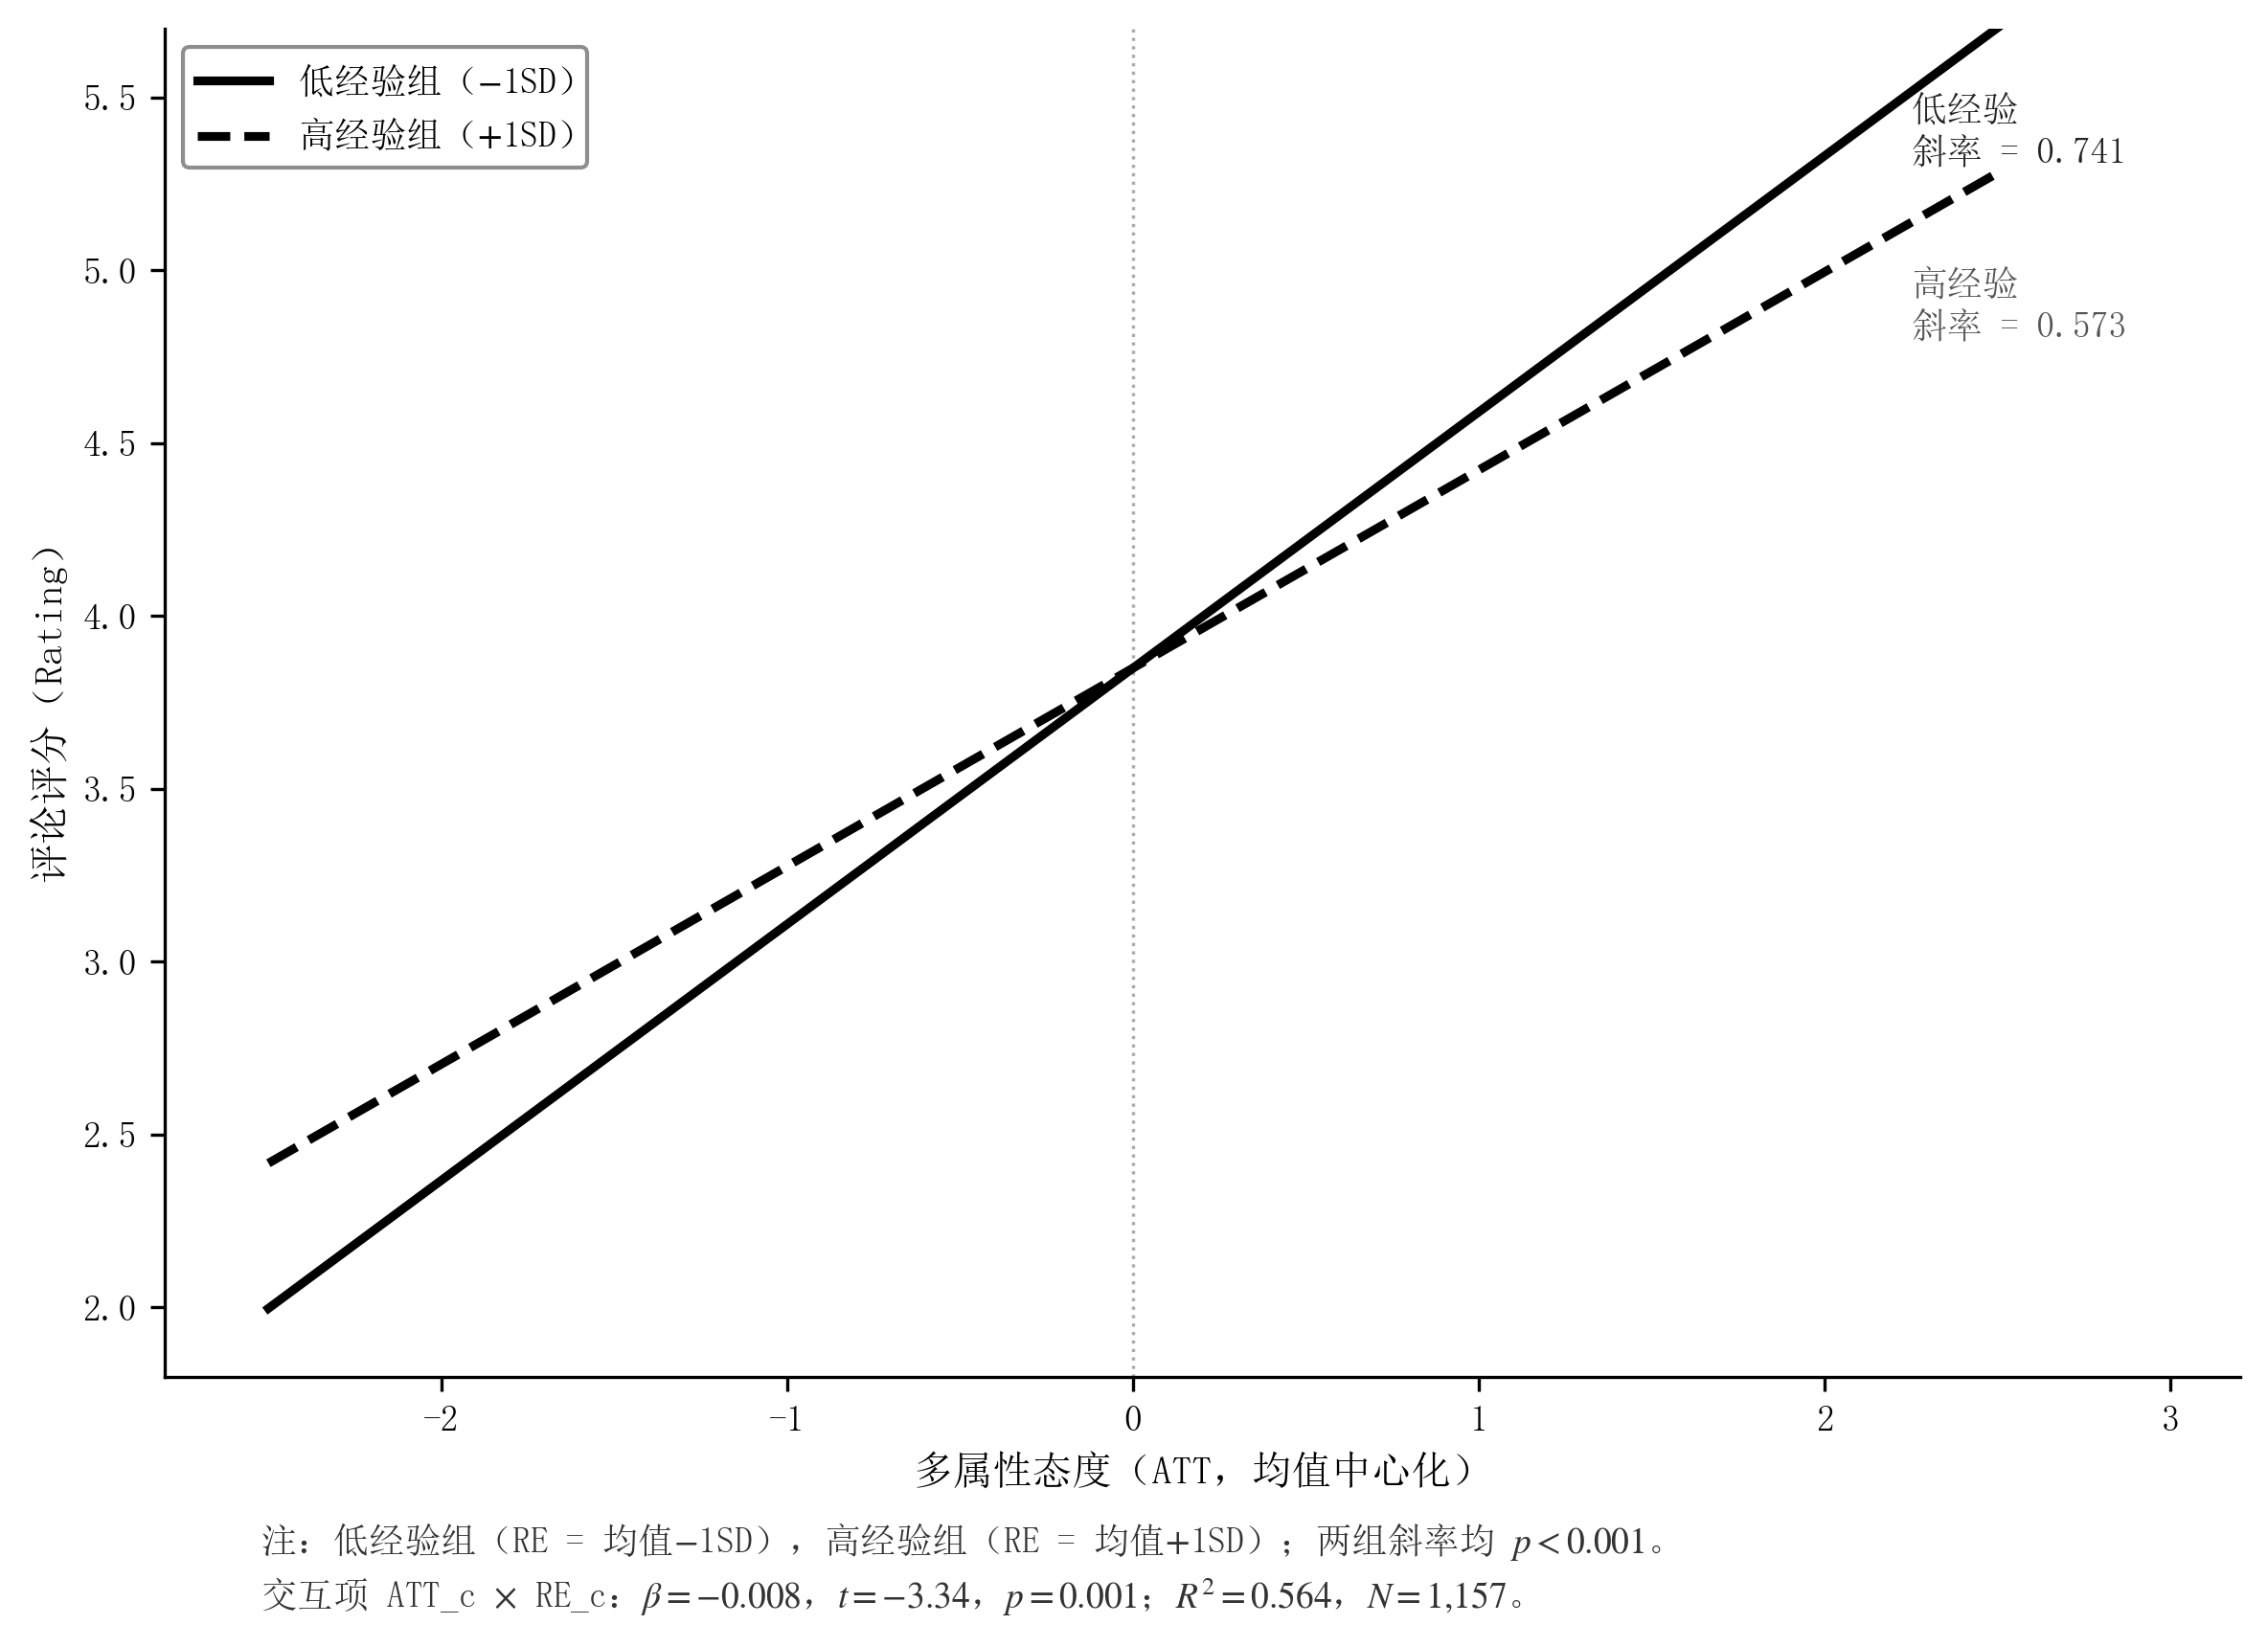
\includegraphics[width=0.9\textwidth]{figures/fig7_2_moderation.png}
\caption{评论者经验对ATT-Rating关系的调节效应（简单斜率分析）}
\label{fig:h2_slopes}
\end{figure}

\subsubsection{H1/H2小结}

H1/H2分析的核心发现：（1）LLM提取的多属性态度（ATT）能够强有力地正向预测评论评分（Rating），有序Logistic回归$\beta=1.867$，$p<0.001$，OLS $R^2=0.560$，证明LLM提取方法具有高预测效度（H1支持）；（2）评论者经验显著负向调节ATT对Rating的预测关系（H2以探索性结果支持），低经验组ATT--Rating斜率更高这一发现挑战了"经验增强一致性"的线性假设，揭示了高经验评论者评价机制的复杂性（详见讨论章节）。

\subsection{H3和H4检验结果}

\subsubsection{选择偏差检验}

使用Welch's $t$ 检验比较BI存在组（$N=298$）与BI缺失组（$N=859$）在ATT均值上的差异：
\begin{itemize}
  \item BI存在组：ATT均值 $= 1.370$（$SD=1.130$）
  \item BI缺失组：ATT均值 $= 0.944$（$SD=1.215$）
  \item $t(441) = 4.604$，$p<0.001$
\end{itemize}

这一显著差异证实存在选择偏差：态度更积极的评论者更可能在评论中表达行为意向。这是H3/H4分析的已知局限性，意味着分析结论仅适用于"明确表达行为意向的评论者"子群，不能推广至全体评论者。

\subsubsection{H3/H4分析变量统计}

H3/H4分析子样本的描述性统计见表\ref{tab:desc_h34}（第六章）。Harman单因子检验显示，ATT和BI（均来自同一评论文本）的单因子解释方差为76.8\%，超过50\%阈值，证实存在同源方差（CMV）问题，分析结论需审慎解读。

\subsubsection{H3检验：ATT正向预测BI}

以BI为因变量，以ATT、Rating、review\_length、helpful\_vote为预测变量，执行OLS回归。

\begin{table}[htbp]
\centering
\caption{H3检验：OLS回归结果（$N=298$）}
\label{tab:h3_ols}
\begin{threeparttable}
\begin{tabular}{@{}lrrrr@{}}
\toprule
变量 & $\beta$ & SE & $t$ & $p$ \\
\midrule
ATT & 0.167 & 0.058 & 2.885 & $0.004$ \\
Rating & 0.368 & 0.065 & 5.660 & $<0.001$ \\
review\_length & 0.001 & 0.000 & 1.823 & $0.069$ \\
helpful\_vote & $-$0.038 & 0.029 & $-$1.317 & $0.189$ \\
\midrule
$R^2$（调整后） & \multicolumn{4}{l}{0.354} \\
\bottomrule
\end{tabular}
\end{threeparttable}
\end{table}

\textbf{H3检验结论}：ATT显著正向预测BI（$\beta=0.167$，$t=2.885$，$p=0.004$），H3获得支持。在同时控制Rating和控制变量的条件下，ATT仍能独立预测行为意向，表明多属性态度对BI具有独立的预测贡献。

\subsubsection{H4检验：ATT的增量效度}

采用层次回归分析（Hierarchical Regression），通过三个嵌套模型检验ATT在控制Rating后的增量预测力（$\Delta R^2$）：

\begin{table}[htbp]
\centering
\caption{H4检验：层次回归分析结果（$N=298$）}
\label{tab:h4_hierarchical}
\begin{threeparttable}
\begin{tabular}{@{}lrrr@{}}
\toprule
 & Model 1 & Model 2 & Model 3 \\
\midrule
控制变量 & & & \\
\quad review\_length & 0.002$^{***}$ & 0.001$^{*}$ & 0.001$^{*}$ \\
\quad helpful\_vote & $-$0.060$^{*}$ & $-$0.041 & $-$0.038 \\
\quad review\_year & $-$0.016 & $-$0.019 & $-$0.020 \\
Rating（核心变量） & & 0.377$^{***}$ & 0.368$^{***}$ \\
ATT（增量变量） & & & 0.167$^{**}$ \\
\midrule
$R^2$ & 0.022 & 0.336 & 0.354 \\
$\Delta R^2$ & & 0.314$^{***}$ & 0.018$^{**}$ \\
$\Delta F$ & & $F=139.8^{***}$ & $F=8.32^{**}$ \\
$p$ for $\Delta F$ & & $<0.001$ & $0.004$ \\
\bottomrule
\end{tabular}
\begin{tablenotes}
\small
\item 注：$^{*}p<0.05$，$^{**}p<0.01$，$^{***}p<0.001$。表中系数为非标准化回归系数（$B$）。
\end{tablenotes}
\end{threeparttable}
\end{table}

\textbf{H4检验结论}：在控制Rating（Model 2 $R^2=0.336$）后，加入ATT（Model 3）使$R^2$提升$\Delta R^2=0.018$（$F=8.32$，$p=0.004$），H4获得支持。尽管$\Delta R^2$的绝对量较小，但其统计显著性表明多属性态度提供了超越单一评分的信息增量，证明多属性分解的独特价值。

图\ref{fig:h4_rsq}展示了三个嵌套模型的$R^2$递增情况及ATT的增量贡献。

\begin{figure}[htbp]
\centering
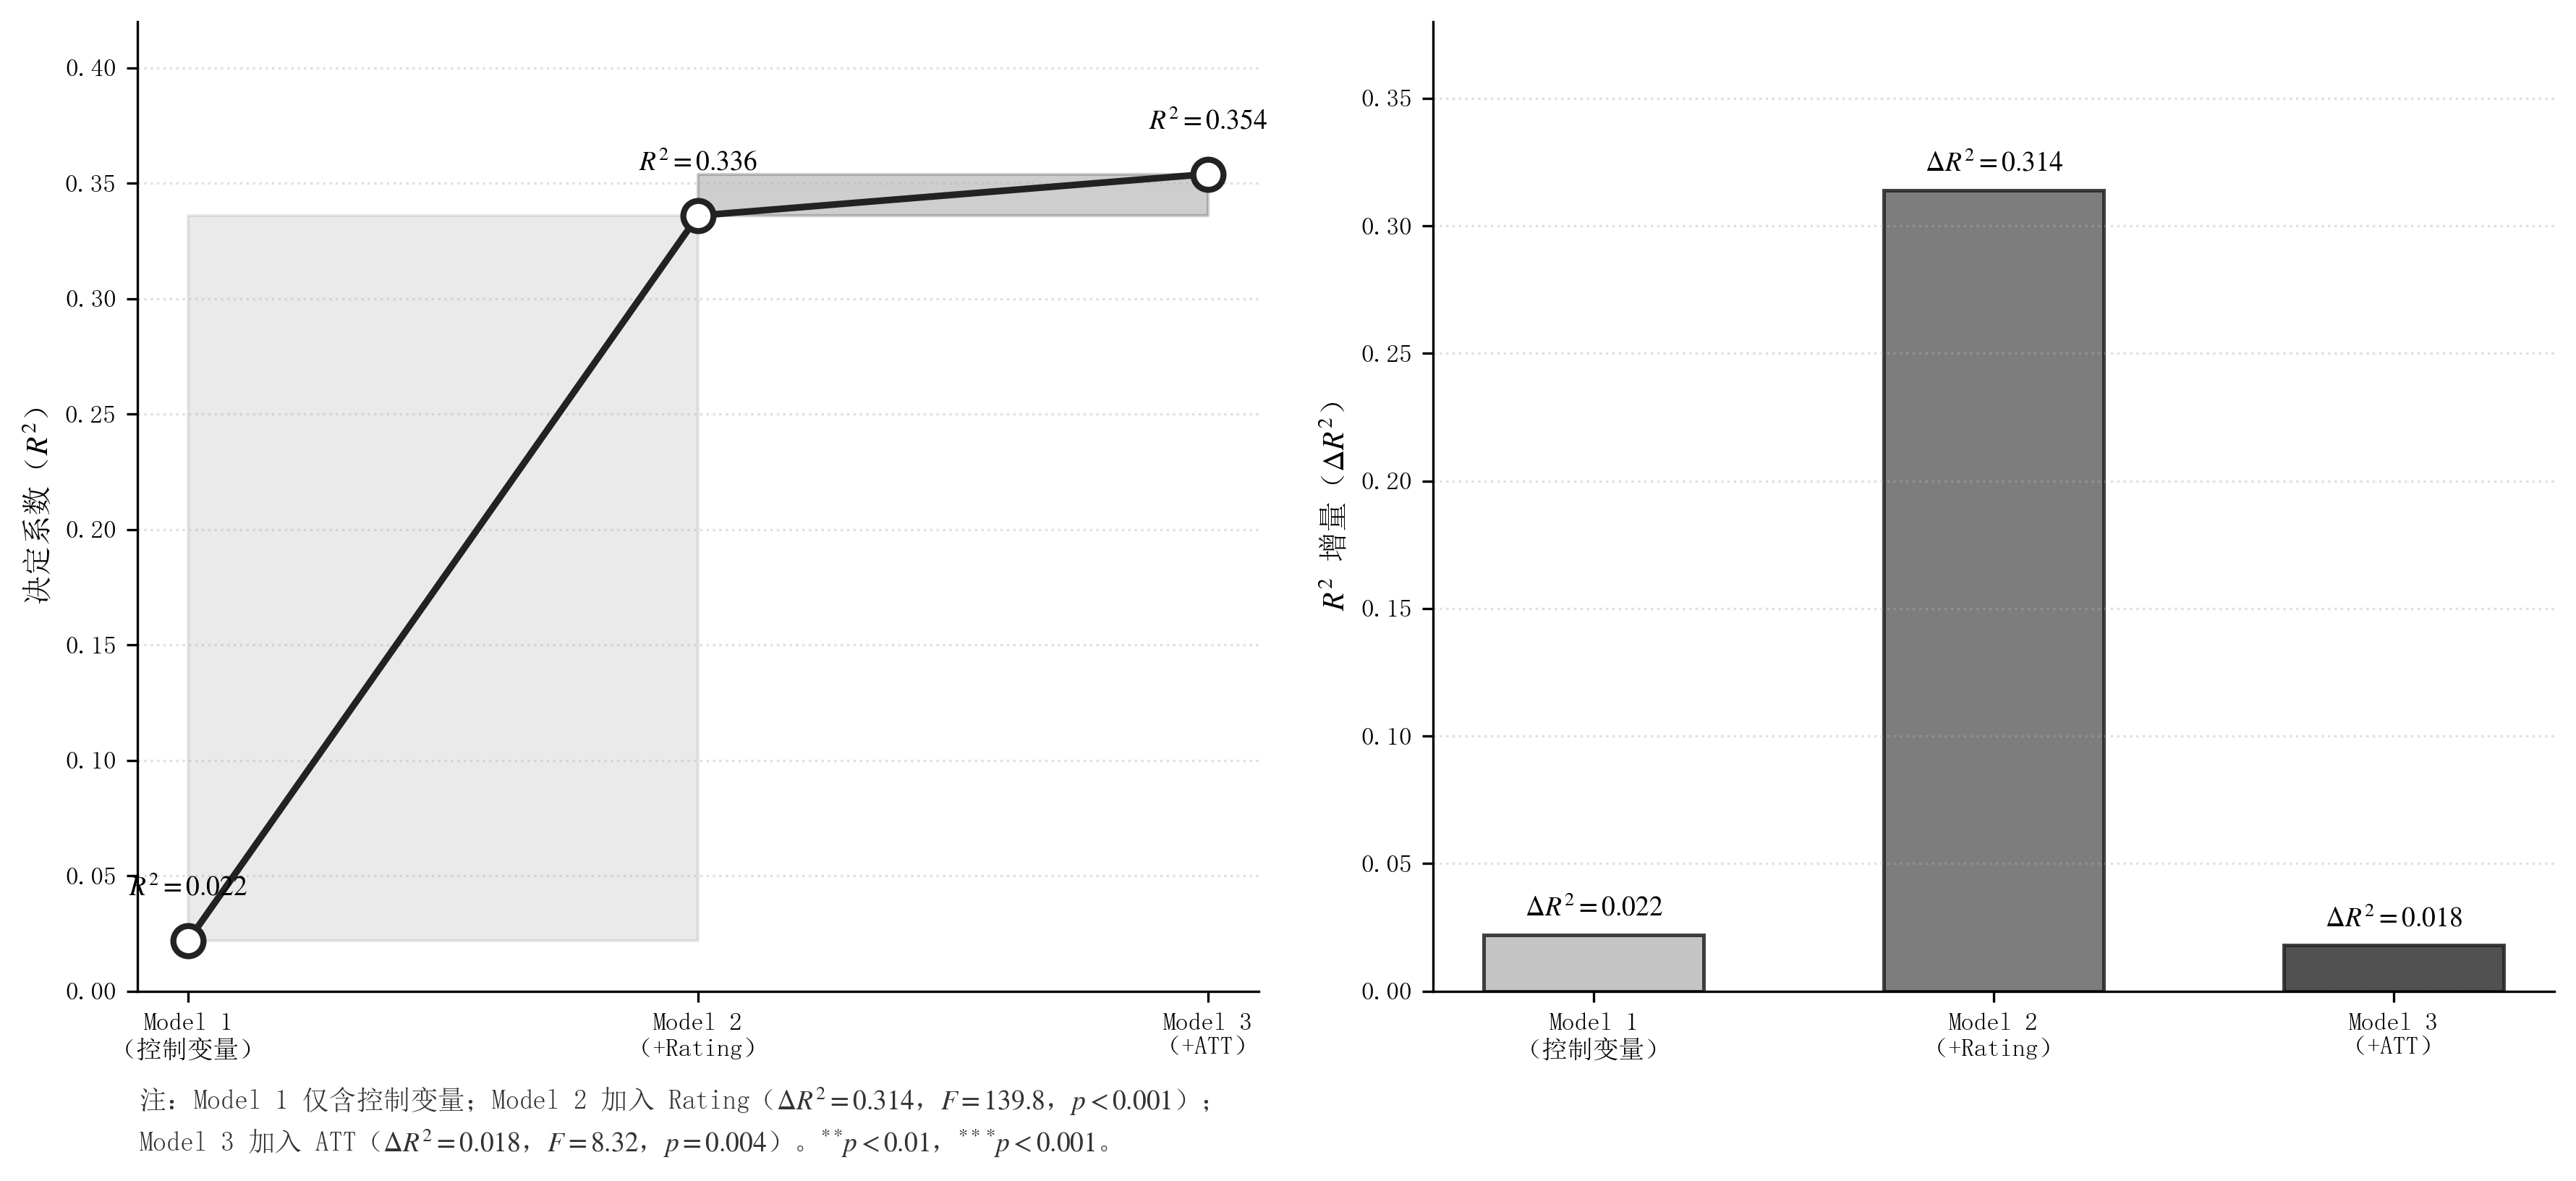
\includegraphics[width=\textwidth]{figures/fig7_3_incremental.png}
\caption{多属性态度（ATT）的增量效度分析}
\label{fig:h4_rsq}
\end{figure}

\subsubsection{H3/H4小结}

H3/H4分析的核心发现：（1）ATT显著正向预测BI（H3支持），$\beta=0.167$，$p=0.004$，与计划行为理论的预测一致；（2）在控制Rating后，ATT对BI仍具有显著的增量预测力（H4支持），$\Delta R^2=0.018$，$p=0.004$，证明多属性态度提供了超越单一总体评分的细粒度信息。需要注意，H3/H4分析存在同源方差（CMV = 76.8\%）和选择偏差（$t=4.60$，$p<0.001$）两项局限，分析结论需在此局限框架下审慎解读。

\clearpage

% ch8_discussion.tex — 第八章 讨论
\section{讨论}

\subsection{H1讨论：ATT对Rating的预测效度}

H1的发现揭示了LLM提取的多属性态度指数与平台客观评分之间的强预测关系（有序Logistic $\beta=1.867$，$p<0.001$；OLS $R^2=0.560$），为"Text as Data"方法论在消费者行为研究中的应用提供了实证支持。这一结果与Mudambi \& Schuff（2010）\cite{mudambi2010}关于评论诊断性的研究形成呼应——该研究发现评论文本的信息深度影响消费者的评分感知，而本研究进一步表明，从文本中系统提取的多属性信念结构本身就与评分存在高度对应（$r=0.722$）。

这里需要回应一个潜在质疑：ATT与Rating的高相关是否意味着两者测量的是同一构念，从而构成"循环论证"？本研究认为不然，理由有三。其一，两者的测量机制根本不同：ATT通过LLM对非结构化文本进行多属性分解得到，Rating是评论者在行为完成后的单次整体判断，信息来源和加工过程均独立；其二，H4的增量效度检验（$\Delta R^2=0.018$，$p=0.004$）证明，在控制Rating之后ATT仍对行为意向有额外预测力，说明两者并不等价；其三，高相关本身正是聚合效度（convergent validity）的体现——若ATT对评分毫无预测力，才应怀疑LLM提取方法的有效性。因此，$r=0.722$既是方法论验证的核心证据，也为后续研究将LLM提取的多属性态度用于评分预测提供了依据。

\subsection{H2讨论：评论者经验的调节效应}

H2的发现揭示了一个在理论上具有启示意义的反向调节模式：低经验评论者的ATT--Rating一致性（简单斜率$=0.741$）反而强于高经验评论者（$0.573$），这与基于Fazio \& Zanna（1978）\cite{fazio1978}直接经验理论"经验增强态度--行为一致性"的预期相悖。

这一发现不应被解读为理论的失效，而是揭示了经验效应在在线评论情境下的特殊作用机制。本研究提出以下解释路径：

\textbf{比较性评价框架的形成。}高经验评论者（Beauty品类评论数多）在长期评论实践中形成了跨产品的参照体系。其评分行为不仅反映对当前产品属性的直接判断，还融入了与竞品、替代品和历史经验的比较性权衡。这种比较性评价框架使ATT（仅基于当前评论文本的属性信念）无法完整解释评分行为，导致两者的对应关系相对松弛。低经验评论者缺乏此类跨产品参照，其评分更直接地映射当前产品体验，ATT与Rating因此保持更高一致性。

\textbf{评分策略的保守化偏移。}Mitchell（2022）\cite{mitchell2022}的研究发现，消费者专业性水平越高，其评分行为越呈现出"保留高分区间"的策略性特征。高经验评论者可能形成了相对固定的评分锚点（如"5星仅授予真正卓越的产品"），即使多属性态度积极，也不轻易给出最高评分，造成ATT与Rating之间的系统性偏差，而这种偏差在低经验评论者中较少出现。

H2的发现对消费者行为研究具有双重理论意义：一方面，它挑战了"经验线性增强态度--行为一致性"的简单假设，表明经验的调节效应是情境依赖的；另一方面，它提示在利用LLM提取多属性态度进行评分预测时，需要将评论者经验纳入模型，对高经验群体的预测精度期望做出相应调整。

\subsection{H3讨论：ATT对BI的直接效应}

H3的发现（$\beta=0.167$，$p=0.004$）与Fishbein \& Ajzen（1975）\cite{fishbein1975}理性行为理论的核心命题一致：态度是行为意向的近端预测变量。在同时控制Rating和控制变量的条件下，ATT仍对BI保持独立预测力，说明多属性分解捕捉到了单一评分无法覆盖的信念结构信息。

需要在方法论框架下审慎解读这一结论。H3/H4分析存在两项已知局限：其一，ATT与BI均提取自同一评论文本，Harman单因子检验（76.8\%$>$50\%阈值）证实存在严重的同源方差（CMV）问题，两者的相关可能被人为放大；其二，BI存在组（$N=298$）的ATT均值（1.370）显著高于BI缺失组（0.944），$t=4.604$，$p<0.001$，选择偏差使子样本的态度分布偏向积极端，H3的效应量可能高于总体真实水平。因此，H3的结论仅适用于"明确在评论中表达行为意向的评论者"这一子群，不宜推广至全体评论者。

\subsection{H4讨论：ATT的增量效度}

H4的发现是本研究最重要的理论贡献之一：在已解释大部分BI方差的Rating（$\Delta R^2=0.314$）之上，ATT仍能提供显著增量预测力（$\Delta R^2=0.018$，$p=0.004$）。

$\Delta R^2=0.018$的绝对量虽小，但其理论意义不应以效应量的大小来衡量，而应以其所揭示的信息增量来理解。评分作为单一整体判断，压缩了消费者态度结构中大量的内部分化信息——例如，"外包装简陋但保湿效果优异"的评论者可能给出4星，其高保湿信念强度与低外观满意度相互抵消后才形成评分，而ATT的多属性分解能够保留这种属性间的结构性差异。正是这部分单一评分所"丢失"的信念结构，构成了ATT对BI的增量预测来源。这一解释与Fishbein多属性态度理论\cite{fishbein1975}的核心论点一致：相比整体态度，属性分解视角能更精确地捕捉消费者行为意向背后的信念机制。

从信息论的视角看，Rating作为单一值已将消费者态度的绝大部分信息压缩其中（Model 2 $R^2=0.336$），剩余可解释的BI方差本就十分有限；ATT能在这一狭小空间中额外捕获1.8\%的方差，恰恰说明多属性分解触及了单维评分无法覆盖的态度结构性差异。换言之，这不是ATT的预测力弱，而是Rating已经很强——ATT在高度压缩的剩余信息空间里仍能挤出显著增量，正是其独立信息价值的体现。

从方法论层面，H4的支持回应了"ATT仅是Rating代理变量"的质疑，证明多属性分解具有独立的信息价值，为在行为预测模型中同时纳入评分与多属性态度提供了依据。

\subsection{方法论讨论：LLM文本提取的可靠性}

LLM可靠性验证结果（ATT计算准确率100\%，幻觉率4.2\%，跨模型重测信度$r=0.892$）表明，在规范的提示词设计（防幻觉约束、few-shot校准、格式强制）下，LLM能够可靠地执行基于Fishbein理论的多属性信念提取任务。

值得关注的是$b_i$信念强度的ICC（0.249），低于0.70的可接受阈值。这一结果并不意味着整体方法失效——$e_i$情感极性的跨模型一致率（97.2\%）和ATT总分的重测信度（$r=0.892$）均达到良好水平，说明信念强度赋值的绝对数值存在模型间差异，但情感方向判断和加权汇总结果保持稳定。其可能的原因是不同LLM在0--3量表的数值校准上缺乏统一参照，这一局限提示未来研究可通过锚定样例（anchor examples）在提示词中统一量表使用标准。

三数据源设计（LLM文本提取/平台客观评分/全品类行为数据）是本研究在方法论上的核心贡献。这一设计将Podsakoff等（2003）\cite{podsakoff2003}提出的程序控制策略与数据来源独立性原则结合，为利用大规模平台数据进行消费者行为研究提供了可复用的CMV控制范式，具有超越本研究情境的方法论推广价值。

\subsubsection{消除CMV的进一步尝试与方法论启示}

为探究能否从根源上消除H3/H4分析的同源方差，本研究事后探索了两种将行为意向操作化为外部行为指标的可能性。

\textbf{方案一（重复购买行为）。}以评论者后续是否再次评论同一产品作为实际回购行为的代理变量。在目标产品（ASIN: B004EDYQX6）的1{,}331条评论中，仅发现7位评论者（涉及15条评论，占总样本1.1\%）有重复评论行为。为排除该比例仅为个案特殊性所致，进一步对同品类评论量最大的产品进行验证：以REVLON One-Step Volumizer（37{,}185条评论）为例，重复评论用户仅319人（0.87\%），且该比例在不同规模的产品中保持高度稳定。即便将分析范围扩大至评论量超过10万条的产品，按0.87\%的结构性比率推算，可获取的重复评论者约870人——虽在统计效力上勉强达标，但该代理指标存在三个根本性的构念效度缺陷：其一，绝大多数消费者回购后不再次评论，``未重复评论''被错误等同于``未回购''，假阴性率极高，系统性地稀释效应量；其二，同一用户对同一产品的多条评论中，相当一部分属于更新评论或补充评论而非独立购买后分别撰写，``重复评论''与``重复购买''之间的构念映射存在根本性缺陷；其三，计划行为理论中行为意向（BI）与实际行为（Behavior）属于不同理论层面的变量\cite{ajzen1991}，意向--行为之间存在已被广泛记录的鸿沟\cite{sheeran2022}，以实际回购行为替代行为意向作为效标，实质上改变了H3/H4的理论检验结构。综合以上分析，方案不可行。

\textbf{方案二（有用票数代理）。}将评论的\texttt{helpful\_vote}（有用票数）作为口碑推荐行为的客观代理。然而，89.0\%的评论未获得任何有用票（极度零膨胀分布），且\texttt{helpful\_vote}在理论上测量的是信息接收者对评论质量的感知，而非评论者自身的行为意向，存在构念上的根本错位，方案同样不可行。

上述探索的结果从反面凸显了三数据源设计的独特价值与严苛的前提条件。它进一步表明，在利用用户生成内容开展行为研究时，能够提前规划并实现测量来源的彻底分离（如H1/H2分析的设计），是一种罕见但关键的方法论优势——其价值正是通过"替代方案均行不通"这一事实而得以量化。这一探索也为未来研究指明了方向：要彻底解决态度--行为意向关系中的CMV问题，可能需要依靠电商平台提供匹配的后续购买行为数据，或采用前瞻性的纵向研究设计。

\clearpage

% ch9_conclusion.tex — 第九章 结论
\section{结论}

\subsection{研究发现总结}

本研究采用大语言模型（DeepSeek-V3.2）从亚马逊平台1{,}331条评论中提取基于Fishbein多属性态度理论的消费者态度指数（$\text{ATT} = \sum b_i \times e_i$），并通过四个假设系统验证其预测效度。

H1/H2分析（$N=1{,}157$）的核心发现：ATT与Rating显著正相关（$r=0.722$，$p<0.001$），有序Logistic回归证实ATT显著正向预测Rating（$\beta=1.867$，$z=19.8$，$p<0.001$），OLS $R^2=0.560$，H1获得支持，表明LLM提取的多属性态度具有良好的预测效度。评论者经验对ATT--Rating关系存在显著负向调节（$\beta=-0.008$，$p=0.001$），低经验评论者的ATT--Rating斜率（0.741）高于高经验评论者（0.573），H2以探索性结果获得支持。这一负向调节方向揭示了高经验评论者在评分时可能引入竞品比较等多维度权衡，使态度与评分的简单对应关系趋于复杂，挑战了"经验线性增强态度--行为一致性"的传统假设。

H3/H4分析（$N=298$）的核心发现：ATT显著正向预测BI（$\beta=0.167$，$p=0.004$），H3获得支持；在控制Rating后ATT仍提供显著增量预测力（$\Delta R^2=0.018$，$F=8.32$，$p=0.004$），H4获得支持。需要注意，H3/H4分析存在同源方差（Harman单因子$=76.8\%$）和选择偏差（$t=4.604$，$p<0.001$）两项局限，结论仅适用于"明确表达行为意向的评论者"子群，不宜推广至全体评论者。

\subsection{理论贡献与管理启示}

\textbf{方法论贡献。}本研究提出并验证了基于LLM的多属性态度提取方法（ATT计算准确率100\%，重测信度$r=0.892$，$e_i$一致率97.2\%），为"Text as Data"研究范式\cite{grimmer2022}在消费者行为研究中的应用提供了方法论基础。三数据源设计（LLM文本提取／平台客观评分／全品类行为数据）从根源上消除了CMV问题\cite{podsakoff2003}，为LLM文本分析研究中的CMV控制提供了可复用范式。H3/H4分析中ATT与BI同源于同一文本（Harman单因子$=76.8\%$）的CMV局限与H1/H2分析的三数据源设计形成鲜明对比，进一步凸显了独立数据源设计的方法论价值。本研究进一步探索了以重复购买行为或有用票数作为BI外部代理的可能性，从数据结构（重复评论比例在不同规模产品中均稳定低于1\%）和构念效度（假阴性率极高、重复评论$\neq$重复购买、意向--行为鸿沟）两个层面系统排除了上述替代方案，从而反证了三数据源设计的不可替代性。

\textbf{理论贡献。}H4证明ATT在控制Rating之后仍对BI具有显著增量预测力（$\Delta R^2=0.018$），回应了"ATT只是Rating代理变量"的质疑，表明多属性分解能够捕捉单一评分所压缩的信念结构信息，支持了Fishbein多属性态度理论\cite{fishbein1975}的区分效度。H2的负向调节发现丰富了消费者专业性理论\cite{mitchell2022}在在线评论情境下的内涵，提示研究者在利用LLM提取的态度变量预测评分行为时，需要将评论者经验纳入调节机制的考量。

\textbf{管理启示。}本研究验证了从评论文本中自动提取多属性态度的可行性，为企业提供了低成本的消费者态度监测工具。H4表明多属性分解提供了单一评分之外的额外信息，企业不应仅依赖评分数据评估产品表现，而应深入分析消费者对各属性的信念结构，识别"高重要性+低满意度"的改进维度。H2提示针对高经验评论者群体，其评分行为涉及更复杂的比较性权衡，企业在解读该群体的评分时应结合多属性信念数据进行综合分析。

\subsection{研究局限与未来展望}

本研究存在以下主要局限。第一，单一产品外部效度局限：本研究仅以伯特小蜜蜂护手霜套装为研究对象，方法的普适性需在更广泛的产品类别和电商平台中验证。第二，H3/H4分析的CMV与选择偏差：ATT与BI同源于同一文本（Harman单因子$=76.8\%$），且BI存在组ATT显著更高（$t=4.604$，$p<0.001$），两项局限共同制约了H3/H4结论的推广范围。第三，$b_i$评估的跨模型稳定性：信念强度ICC$=0.249$低于可接受阈值，不同LLM在0--3量表的数值校准上缺乏统一参照，影响了方法的可复现性。第四，reviewer\_experience的代理效度：以品类评论总数衡量消费者专业性存在局限，其与评论质量指标（$r$均接近0）的弱相关提示该代理指标有待改进。第五，H2调节方向的解释边界：H2的负向调节方向虽以探索性假设获得支持，但本研究对其机制的解释（比较性评价框架、评分策略保守化）属于事后推演，无法区分"负向调节确实反映了经验导致评价复杂化"与"反向结果部分源于代理指标局限或样本结构"两种可能。未来研究需通过更直接的消费者专业性测量手段和预先注册的假设对这一调节方向进行独立验证。

未来研究可沿三个方向推进：其一，将LLM多属性态度提取方法扩展至多产品类别、多语言和多平台，检验方法的稳健性；其二，采用独立数据源或实验设计改进H3/H4分析的CMV控制，并通过倾向得分匹配等方法缓解选择偏差；其三，探索基于规则或混合模型的$b_i$赋值方案，提高信念强度评估的跨模型一致性，同时在Fishbein理论框架内整合主观规范、感知行为控制等变量，构建更完整的行为预测模型。

\clearpage

% ---------- 参考文献 ----------
{
\ctexset{section/format = \zihao{-3}\heiti\centering}
\zihao{5}
\printbibliography[
  title  = {参考文献},
  heading = bibintoc,
]
}
\clearpage

% ---------- 附录 ----------
\appendix
\renewcommand{\thesection}{\Alph{section}}
{
\ctexset{section/format = \zihao{-3}\heiti\centering}
% appendix.tex — 附录
\section*{附录}
\addcontentsline{toc}{section}{附录}

\subsection*{附录11.1\quad 项目文件结构}

\begin{verbatim}
bi_ye_she_ji/
├── data/                          # 数据文件夹
│   ├── reviews_B004EDYQX6.jsonl  # 原始评论数据（1331条）
│   ├── cleaned_reviews.csv        # 清洗后的数据（1331条，含未验证购买）
│   └── final_analysis_data.csv    # 最终分析数据（1331条）
├── code/                          # 代码文件夹
│   ├── config.py                  # API配置
│   ├── data_preprocessing.py      # 数据预处理
│   ├── variable_extraction.py     # 变量提取（API调用）
│   ├── load_product_metadata.py   # 商品元数据加载
│   └── test_extraction.py         # 小批量测试脚本
└── output/                        # 输出文件夹
    └── figures/                   # 图表文件夹
\end{verbatim}

\subsection*{附录11.2\quad 核心代码模块说明}

\subsubsection*{11.2.1\quad 数据预处理模块}

\textbf{功能}：将原始JSON评论数据清洗为规整的CSV文件。

\textbf{主要函数}：
\begin{itemize}
  \item \texttt{remove\_html\_tags(text)}：移除HTML标签
  \item \texttt{preprocess\_reviews(input\_file, output\_file)}：数据预处理主函数
\end{itemize}

\textbf{处理步骤}：
\begin{enumerate}
  \item 读取JSONL文件
  \item 合并\texttt{title}和\texttt{text}字段
  \item 移除HTML标签
  \item 生成\texttt{review\_id}
  \item 保存为CSV
\end{enumerate}

\subsubsection*{11.2.2\quad 变量提取模块}

\textbf{功能}：通过大模型API提取消费者信念、评价、强度和行为意向。

\textbf{主要函数}：
\begin{itemize}
  \item \texttt{extract\_beliefs\_and\_evaluation(full\_text, product\_metadata)}：提取信念与评价
  \item \texttt{assess\_belief\_strength(belief\_text, review\_context, review\_length)}：评估信念强度
  \item \texttt{extract\_behavioral\_intention(full\_text)}：提取行为意向
  \item \texttt{main\_extraction\_pipeline()}：主流程函数
\end{itemize}

\textbf{关键特性}：
\begin{itemize}
  \item 支持断点续传
  \item 自动错误处理和重试
  \item 每10条保存临时结果
  \item 支持商品元数据增强
\end{itemize}

\subsubsection*{11.2.3\quad 商品元数据加载模块}

\textbf{功能}：从元数据文件中加载商品信息。

\textbf{主要函数}：
\begin{itemize}
  \item \texttt{load\_product\_metadata(metadata\_file, product\_id)}：加载商品元数据
  \item \texttt{format\_metadata\_for\_prompt(metadata)}：格式化元数据用于提示词
\end{itemize}

\subsection*{附录11.3\quad 数据文件说明}

\subsubsection*{11.3.1\quad cleaned\_reviews.csv}

\textbf{格式}：CSV文件，UTF-8编码。

\textbf{列说明}：
\begin{itemize}
  \item \texttt{review\_id}：评论唯一标识符（R0001, R0002, \ldots）
  \item \texttt{full\_text}：完整评论文本（title + text，已移除HTML标签）
  \item \texttt{rating}：产品评分（1--5分）
\end{itemize}

\textbf{行数}：1{,}331行（包含全部评论，不以 verified\_purchase 过滤）。

\subsubsection*{11.3.2\quad final\_analysis\_data.csv}

\textbf{格式}：CSV文件，UTF-8编码。

\textbf{列说明}：
\begin{itemize}
  \item \texttt{review\_id}：评论唯一标识符
  \item \texttt{ATT}：态度指数（$\text{ATT} = \Sigma(b_i \times e_i)$）
  \item \texttt{BI}：行为意向（0--3整数）
  \item \texttt{rating}：产品评分（1--5分）
  \item \texttt{reviewer\_experience}：评论者经验（Beauty品类历史评论总数）
  \item \texttt{beliefs}：JSON格式的信念提取原始数据，含$b_i$（信念强度，0.4--1.0）、$e_i$（情感极性，$-1/0/+1$）、\texttt{type}（信念类型）字段
\end{itemize}

\textbf{行数}：1{,}331行（包含已验证购买和未验证购买评论）。

\textbf{数据质量}：ATT完整率86.9\%（$N=1{,}157$），BI完整率22.4\%（$N=298$），rating字段100\%完整，ATT取值范围为$-4.1$至$4.6$，BI取值范围为0--3，rating取值范围为1--5。

\subsection*{附录11.4\quad 技术环境}

\subsubsection*{11.4.1\quad Python环境}

\textbf{Python版本}：3.7+

\textbf{主要依赖包}：
\begin{itemize}
  \item \texttt{pandas} $\geq$ 1.4.0
  \item \texttt{openai} $\geq$ 1.0.0
  \item \texttt{statsmodels} $\geq$ 0.13.0
  \item \texttt{scikit-learn} $\geq$ 1.0.0
  \item \texttt{matplotlib} $\geq$ 3.5.0
  \item \texttt{seaborn} $\geq$ 0.11.0
  \item \texttt{scipy} $\geq$ 1.9.0
\end{itemize}

\subsubsection*{11.4.2\quad API配置}

\textbf{API提供商}：便携AI聚合API平台

\textbf{BASE\_URL}：\texttt{https://api.bianxie.ai/v1}

\textbf{模型}：\texttt{deepseek-chat}

\textbf{API延迟}：1.0秒/次（可根据配额调整）

\subsection*{附录11.5\quad 质量控制措施}

\begin{enumerate}
  \item \textbf{数据筛选}：保留全部1{,}331条评论（包含已验证与未验证购买），verified\_purchase与ATT相关系数$r=0.032$（$p=\text{ns}$），对分析结果影响可忽略。
  \item \textbf{文本清洗}：移除HTML标签，清理格式，确保文本质量。
  \item \textbf{API调用质量控制}：自动重试机制（最多3次）；API延迟控制（避免速率限制）；错误处理和日志记录。
  \item \textbf{提取结果验证}：JSON格式验证；数值范围检查（ATT、BI、rating）；小批量测试和人工核对。
  \item \textbf{断点续传}：每10条保存临时结果，支持中断后继续，避免数据丢失。
\end{enumerate}

\subsection*{附录11.6\quad 研究伦理说明}

本研究使用的数据来自亚马逊电商平台的公开评论数据，所有数据均为公开可获取的信息。研究过程中：

\begin{enumerate}
  \item \textbf{数据匿名化}：研究仅使用评论内容，不涉及用户个人身份信息。
  \item \textbf{数据使用}：数据仅用于学术研究，不用于商业用途。
  \item \textbf{数据保护}：所有数据文件存储在本地，不对外公开。
  \item \textbf{研究目的}：本研究旨在理解消费者行为，为学术研究和企业实践提供参考。
\end{enumerate}

}

% ---------- 致谢 ----------
{
\ctexset{section/format = \zihao{-3}\heiti\centering}
% acknowledgment.tex — 致谢
\clearpage
\section*{致\quad 谢}
\addcontentsline{toc}{section}{致谢}

{\zihao{-4}\songti

[Acknowledgment content has been redacted in the public repository version.]

}

}

% ============================================================
\end{document}
% ============================================================
